\documentclass[12pt]{article}

\usepackage[margin=1in]{geometry}
\usepackage{amsfonts,amssymb,amsthm,amsmath,graphicx}
\usepackage{float}
\usepackage{listings}
\usepackage{hyperref}
\usepackage{verbatim}
\usepackage{mathtools}
\usepackage{enumitem}
\usepackage{xcolor}

\hypersetup{
    colorlinks,
    linkcolor={red!50!black},
    citecolor={blue!50!black},
    urlcolor={blue!80!black}
}

\definecolor{boxbackground}{rgb}{1,0.976, 0.882}

\lstset{
    language=Python,
    basicstyle=\scriptsize\ttfamily,
    keywordstyle=\color{blue}\ttfamily,
    stringstyle=\color{red}\ttfamily,
    commentstyle=\color{green!50!black}\ttfamily,
    frame=single,
    breaklines=true,
    postbreak=\raisebox{0ex}[0ex][0ex]{\ensuremath{\color{violet}\hookrightarrow\space}},
    backgroundcolor = \color{boxbackground},
    showspaces=false,
    showstringspaces=false,
}

\newcommand{\N}{\mathbb{N}}
\newcommand{\Z}{\mathbb{Z}}
\newcommand{\R}{\mathbb{R}}
\newcommand{\Q}{\mathbb{Q}}
\newcommand{\e}{\epsilon}
\newcommand{\C}{\mathbb{C}}
\newcommand{\norm}[1]{\left\lVert#1\right\rVert}
\newcommand{\li}[1]{\lstinline[prebreak=]!#1!}

\begin{document}
\title{Fake News on Facebook}
\author{Marissa Graham- CS 401R Final Project}

\maketitle

\section*{Introduction}

Fake news has become especially relevant recently as a result of the 2016 U.S. presidential election, and Facebook and Google are both attempting to fight it. Efforts include economic disincentives to publish such stories, tools to help media consumers identify fake news and be skeptical of what they read, and attempts to stop the viral spread of fake news.

While machine learning tools cannot force people to be more skeptical of what they read or to stop trusting purveyors of fake news, being able to predict with some accuracy whether certain posts are likely to be fake--without manual human supervision--is a necessary step towards building tools to curb the spread of fake news.

In this project, we attempt to predict the truthfulness rating of fact-checked posts from various news outlet pages on Facebook based on the page, page type, post type, and the number of shares, reactions, and comments on the post.

The dataset used is a publicly available \texttt{.csv} file sponsored by Buzzfeed News, which can be found here: \url{https://github.com/BuzzFeedNews/2016-10-facebook-fact-check/blob/master/data/facebook-fact-check.csv} and which contains 2284 Facebook posts by various news outlet pages between September 19th and September 27th of 2016. The methodology used to obtain the dataset and rate each post is described in the article which the dataset was created to support, which can be found here: \url{https://www.buzzfeed.com/craigsilverman/partisan-fb-pages-analysis?utm_term=.pw5olzemMP#.nvdpM7LDqB}.


\section*{Problem Discussion}

This dataset attempts to classify posts into four categories: ``mostly false", ``mixture of true and false", ``mostly true", and ``no factual content" for posts which were satirical, opinion-driven, or otherwise lacked a factual claim. We have this rating information for the entire dataset, so this is a supervised classification problem. 

Superficially, this is most similar to the Gaussian process regression and recommender system labs, in that we are given data with certain features and attempt to make predictions based on some of the features. Since this dataset originated for the purpose of generating various statistics about these posts and not for prediction competitions, it is unclear what other approaches have been tried on similar data. Based on course lectures, the most promising approaches seem to be Gaussian process regression and Naive Bayes classification. 

\section*{Dataset Exploration}
For each post in the dataset, we have an \texttt{account\_id} (unique to each page), a unique \texttt{post\_id} and \texttt{Post URL}, and then the features of the most interest to us are as follows:

\begin{itemize}[noitemsep,nolistsep]
\item \texttt{Category}: mainstream, right, or left
\item \texttt{Page}: ABC News Politics, Addicting Info, CNN Politics, Eagle Rising, Freedom Daily, Occupy Democrats, Politico, Right Wing News, The Other 98\%
\item \texttt{Date Published}: 2016-09-19 through 2016-09-27
\item \texttt{Post Type}: video, link, text, or photo
\item \texttt{Rating}: mostly false, mostly true, mixture of true and false, or no factual content
\item Engagement counts: \texttt{share\_count}, \texttt{reaction\_count}, and \texttt{comment\_count}
\end{itemize}

First, we check to see the overall distribution of truthfulness ratings. The majority (73.1\% of) posts were ``mostly true", with ``mixture of true and false" and ``no factual content" about on par with each other at 10.7\% and 11.6\%, respectively. 4.6\% of posts were ``mostly false", which is fortunately smaller than any other rating, but still disturbingly high for posts from supposed news outlets.

We then visualize the distribution of truthfulness ratings over various other features of the data in order to get a sense of which features most strongly influence the truthfulness rating of the post.

\begin{figure}[H] 
    \centering
    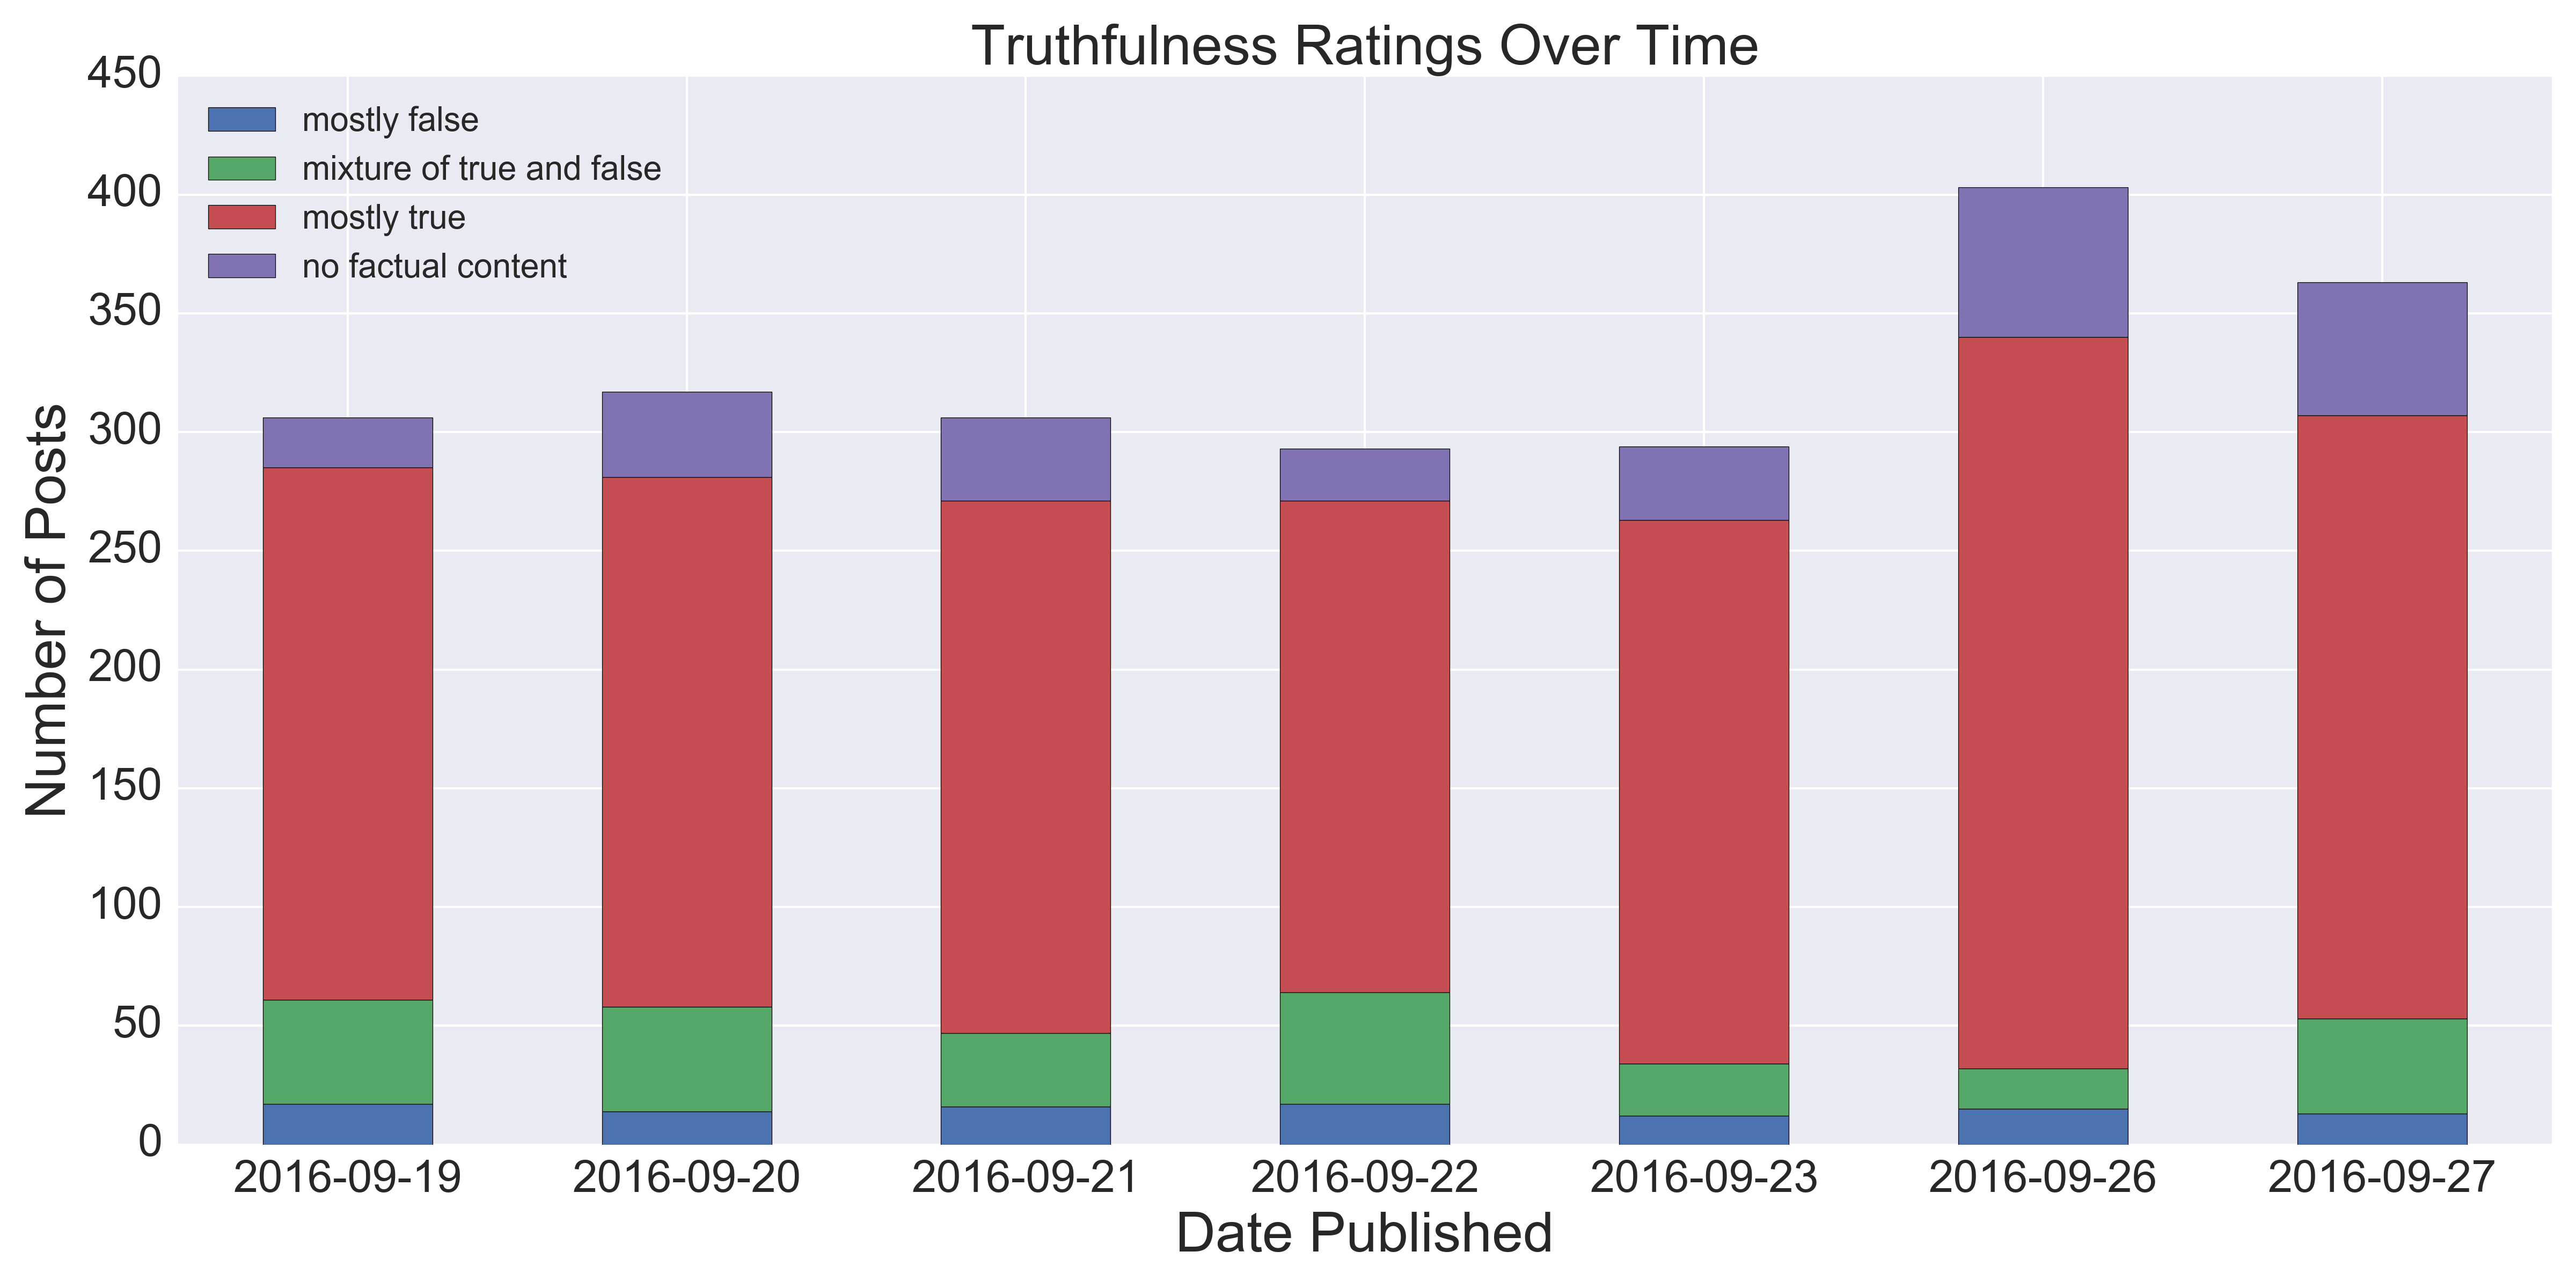
\includegraphics[width=\textwidth]{ratings_distribution_over_time.png}
\end{figure}

While this is too short a time frame to notice any long term trends in the prevalence of fake news, we do notice a spike in the overall number of posts on September 26th, which corresponds to the first presidential debate. The majority of this increase seems to be in the form of non-factual content, followed by a spike in misleading news the next day. Overall, however, truthfulness ratings do not seem to be too strongly correlated with their day of appearance in this dataset.

\begin{figure}[H] 
    \centering
    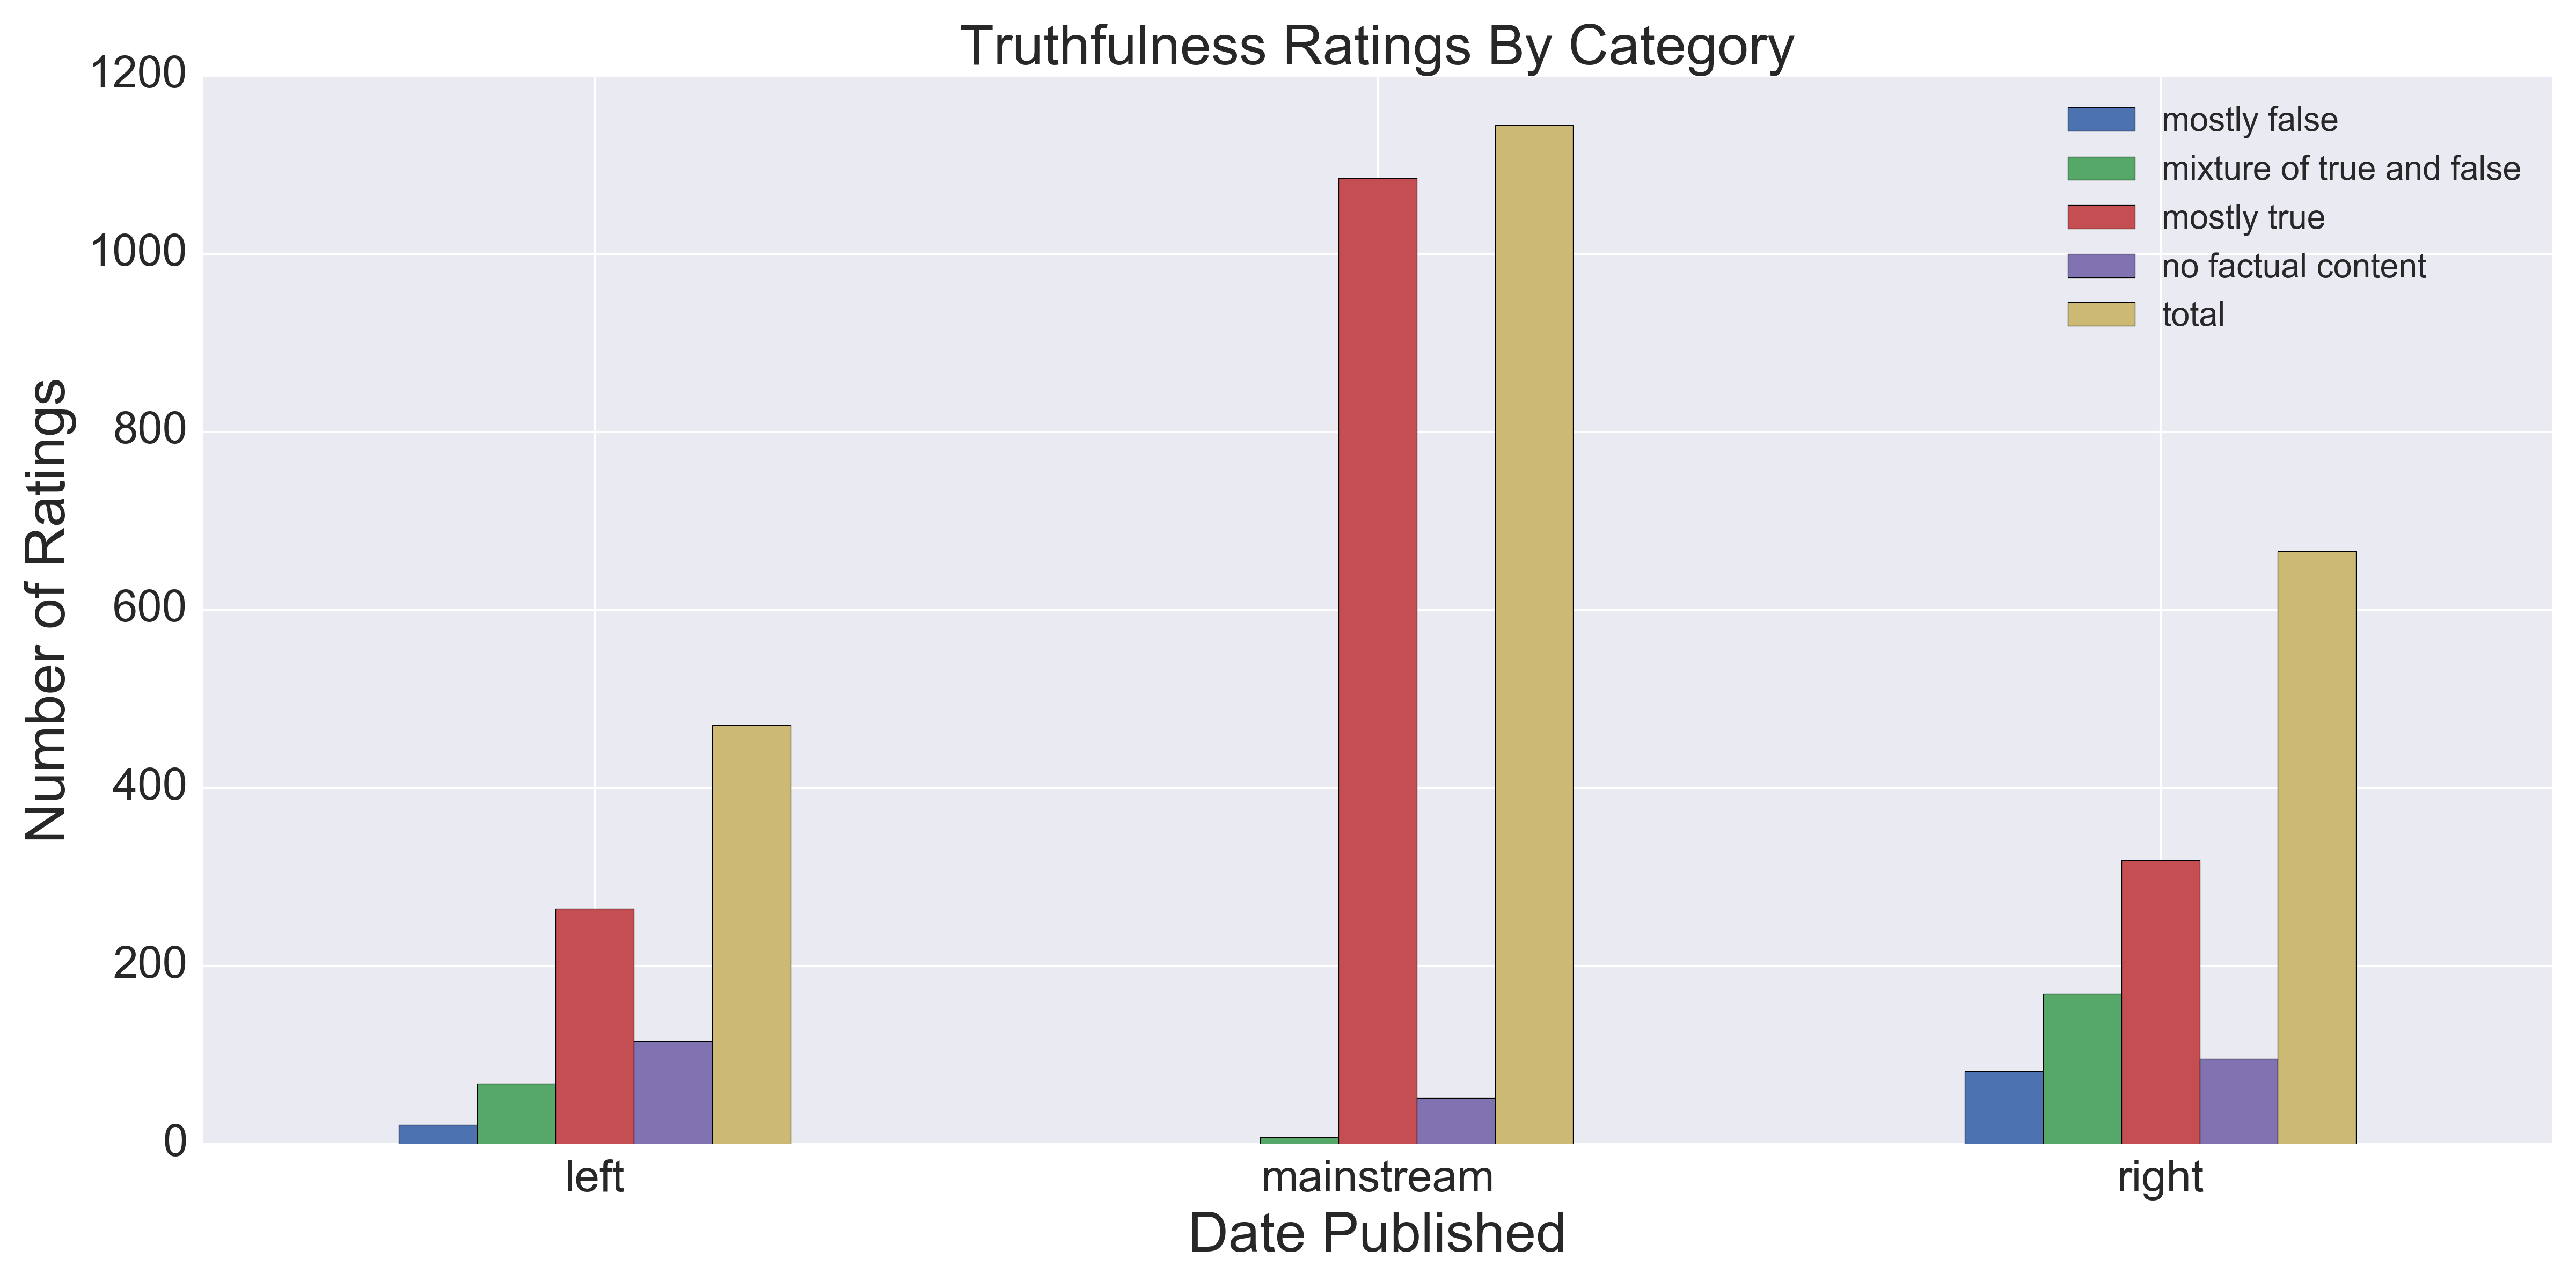
\includegraphics[width=\textwidth]{ratings_distribution_by_category.png}
\end{figure}

We see a much stronger effect in truthfulness when looking at categories. Mainstream news outlets are highly unlikely to post fake news, with not a single incident observed in the data. Left-wing outlets are less likely to post false or misleading content, but are more likely to post non-factual content. 

Looking further into the page breakdown, we notice that Politico is the most prolific and most trustworthy of the news outlets in our dataset, while Eagle Rising and Occupy Democrats are the least trustworthy in terms of what percentage of their content is considered ``mostly true". However, the difference in trustworthiness amont categories of outlets is not as notable as the difference in trustworthiness between categories of outlets.

\begin{figure}[H] 
    \centering
    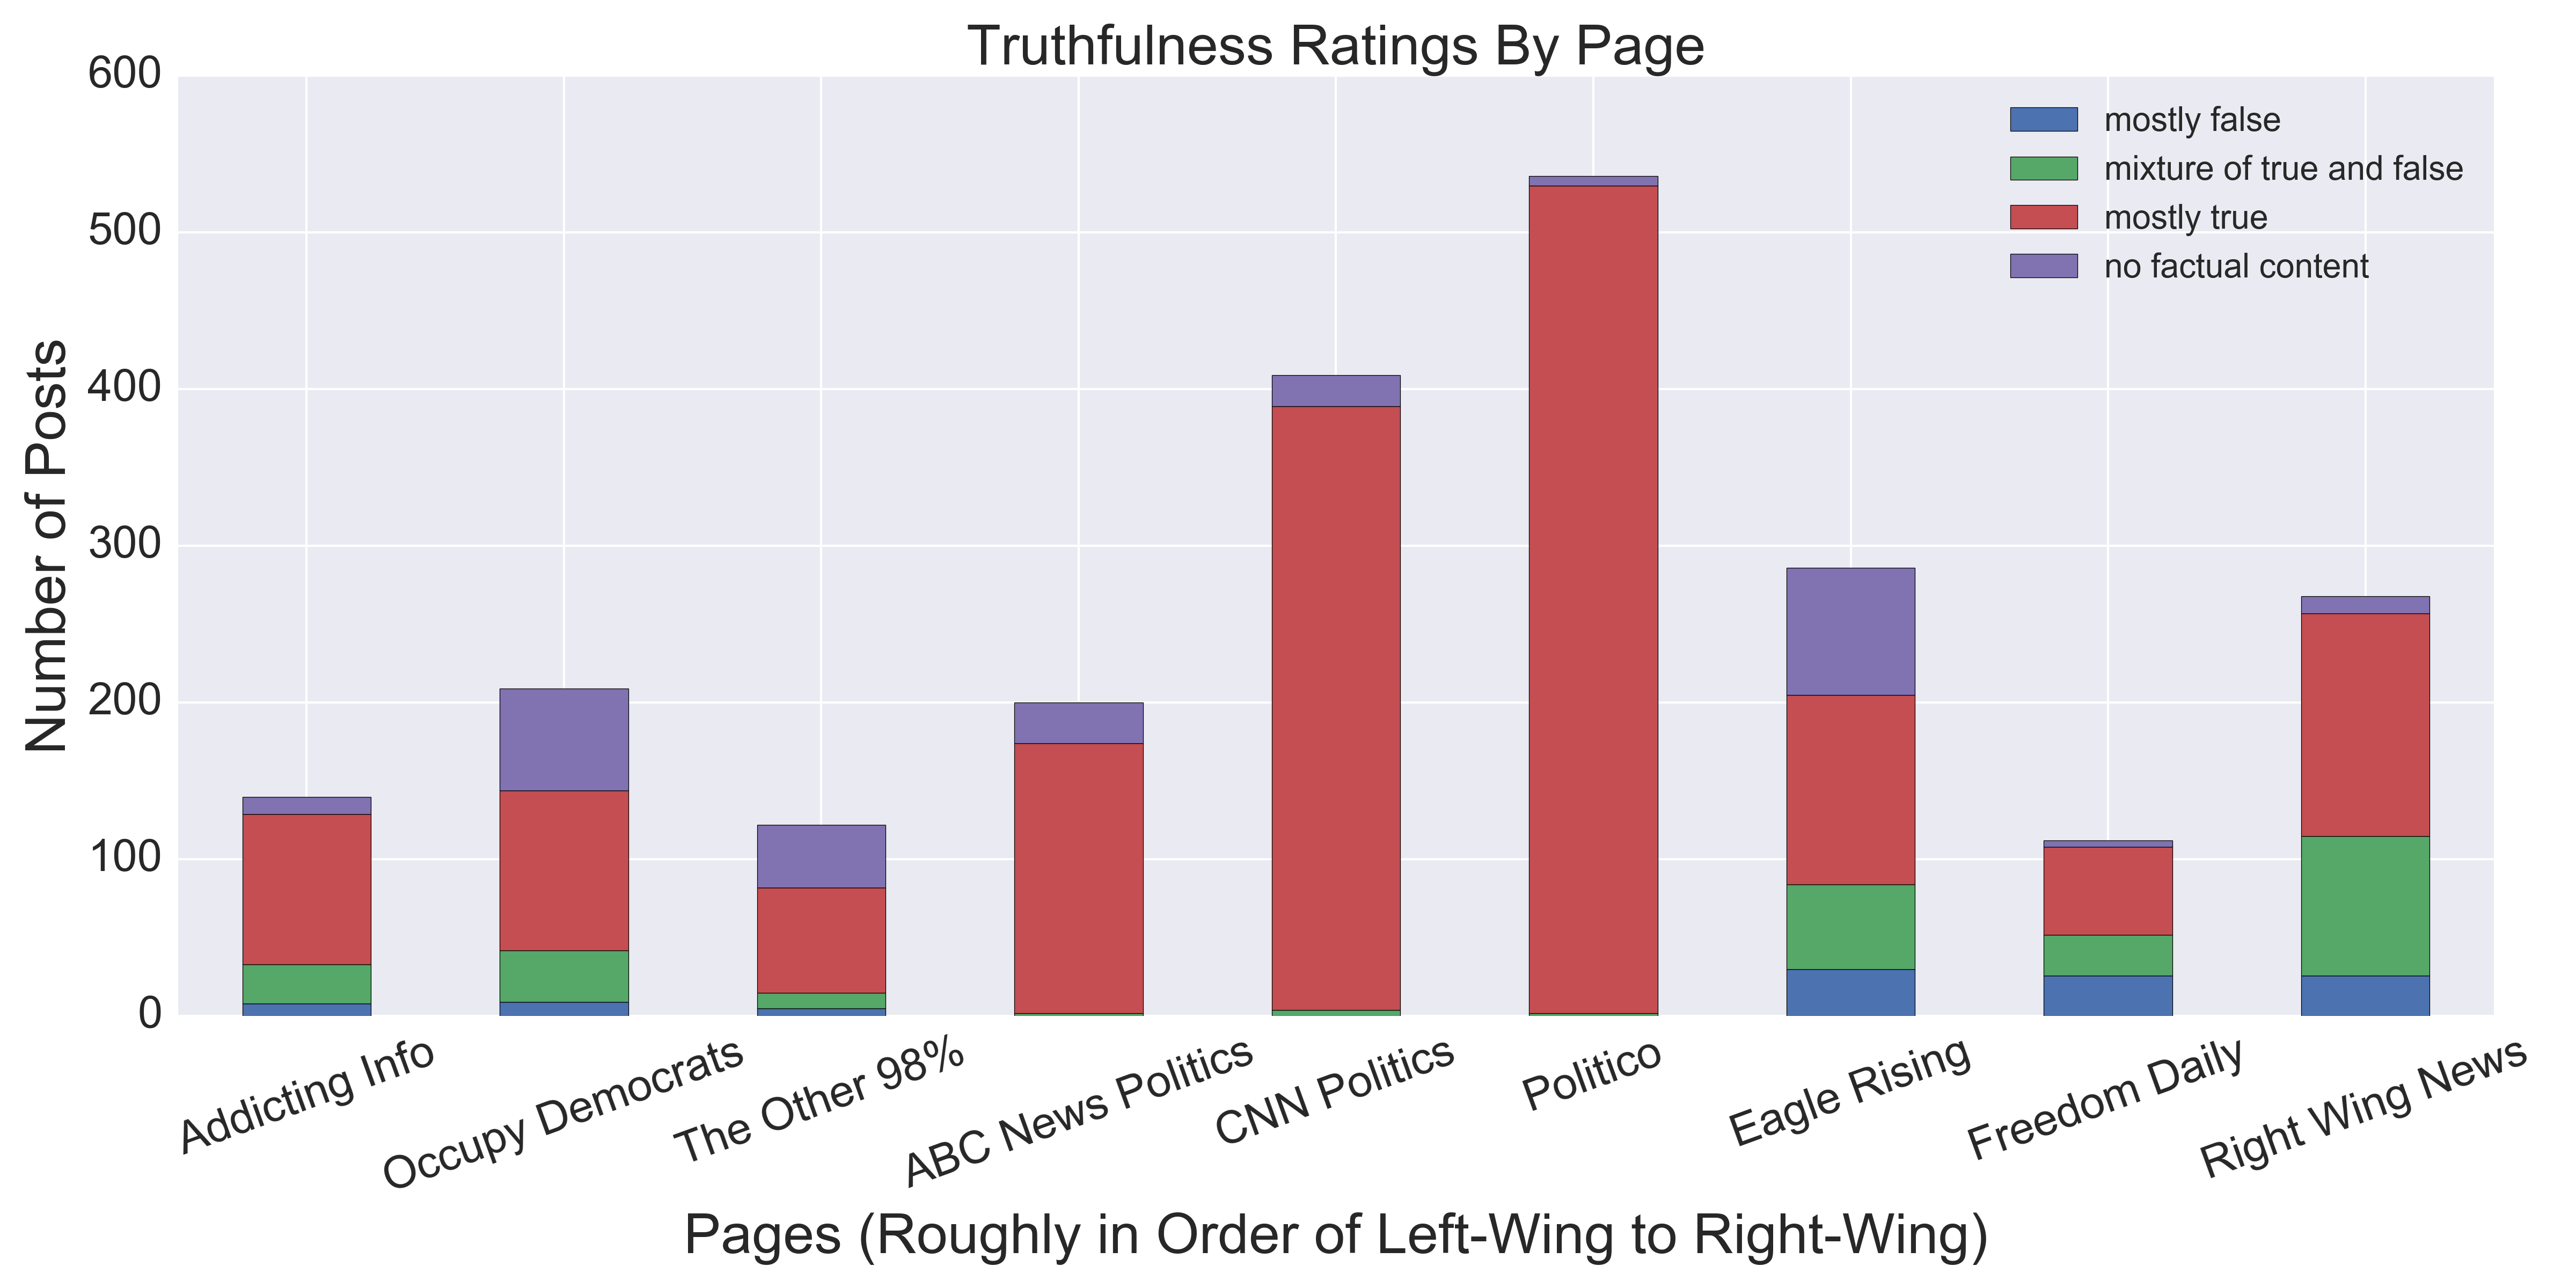
\includegraphics[width=\textwidth]{ratings_distribution_by_page.png}
\end{figure}

\begin{figure}[H] 
    \centering
    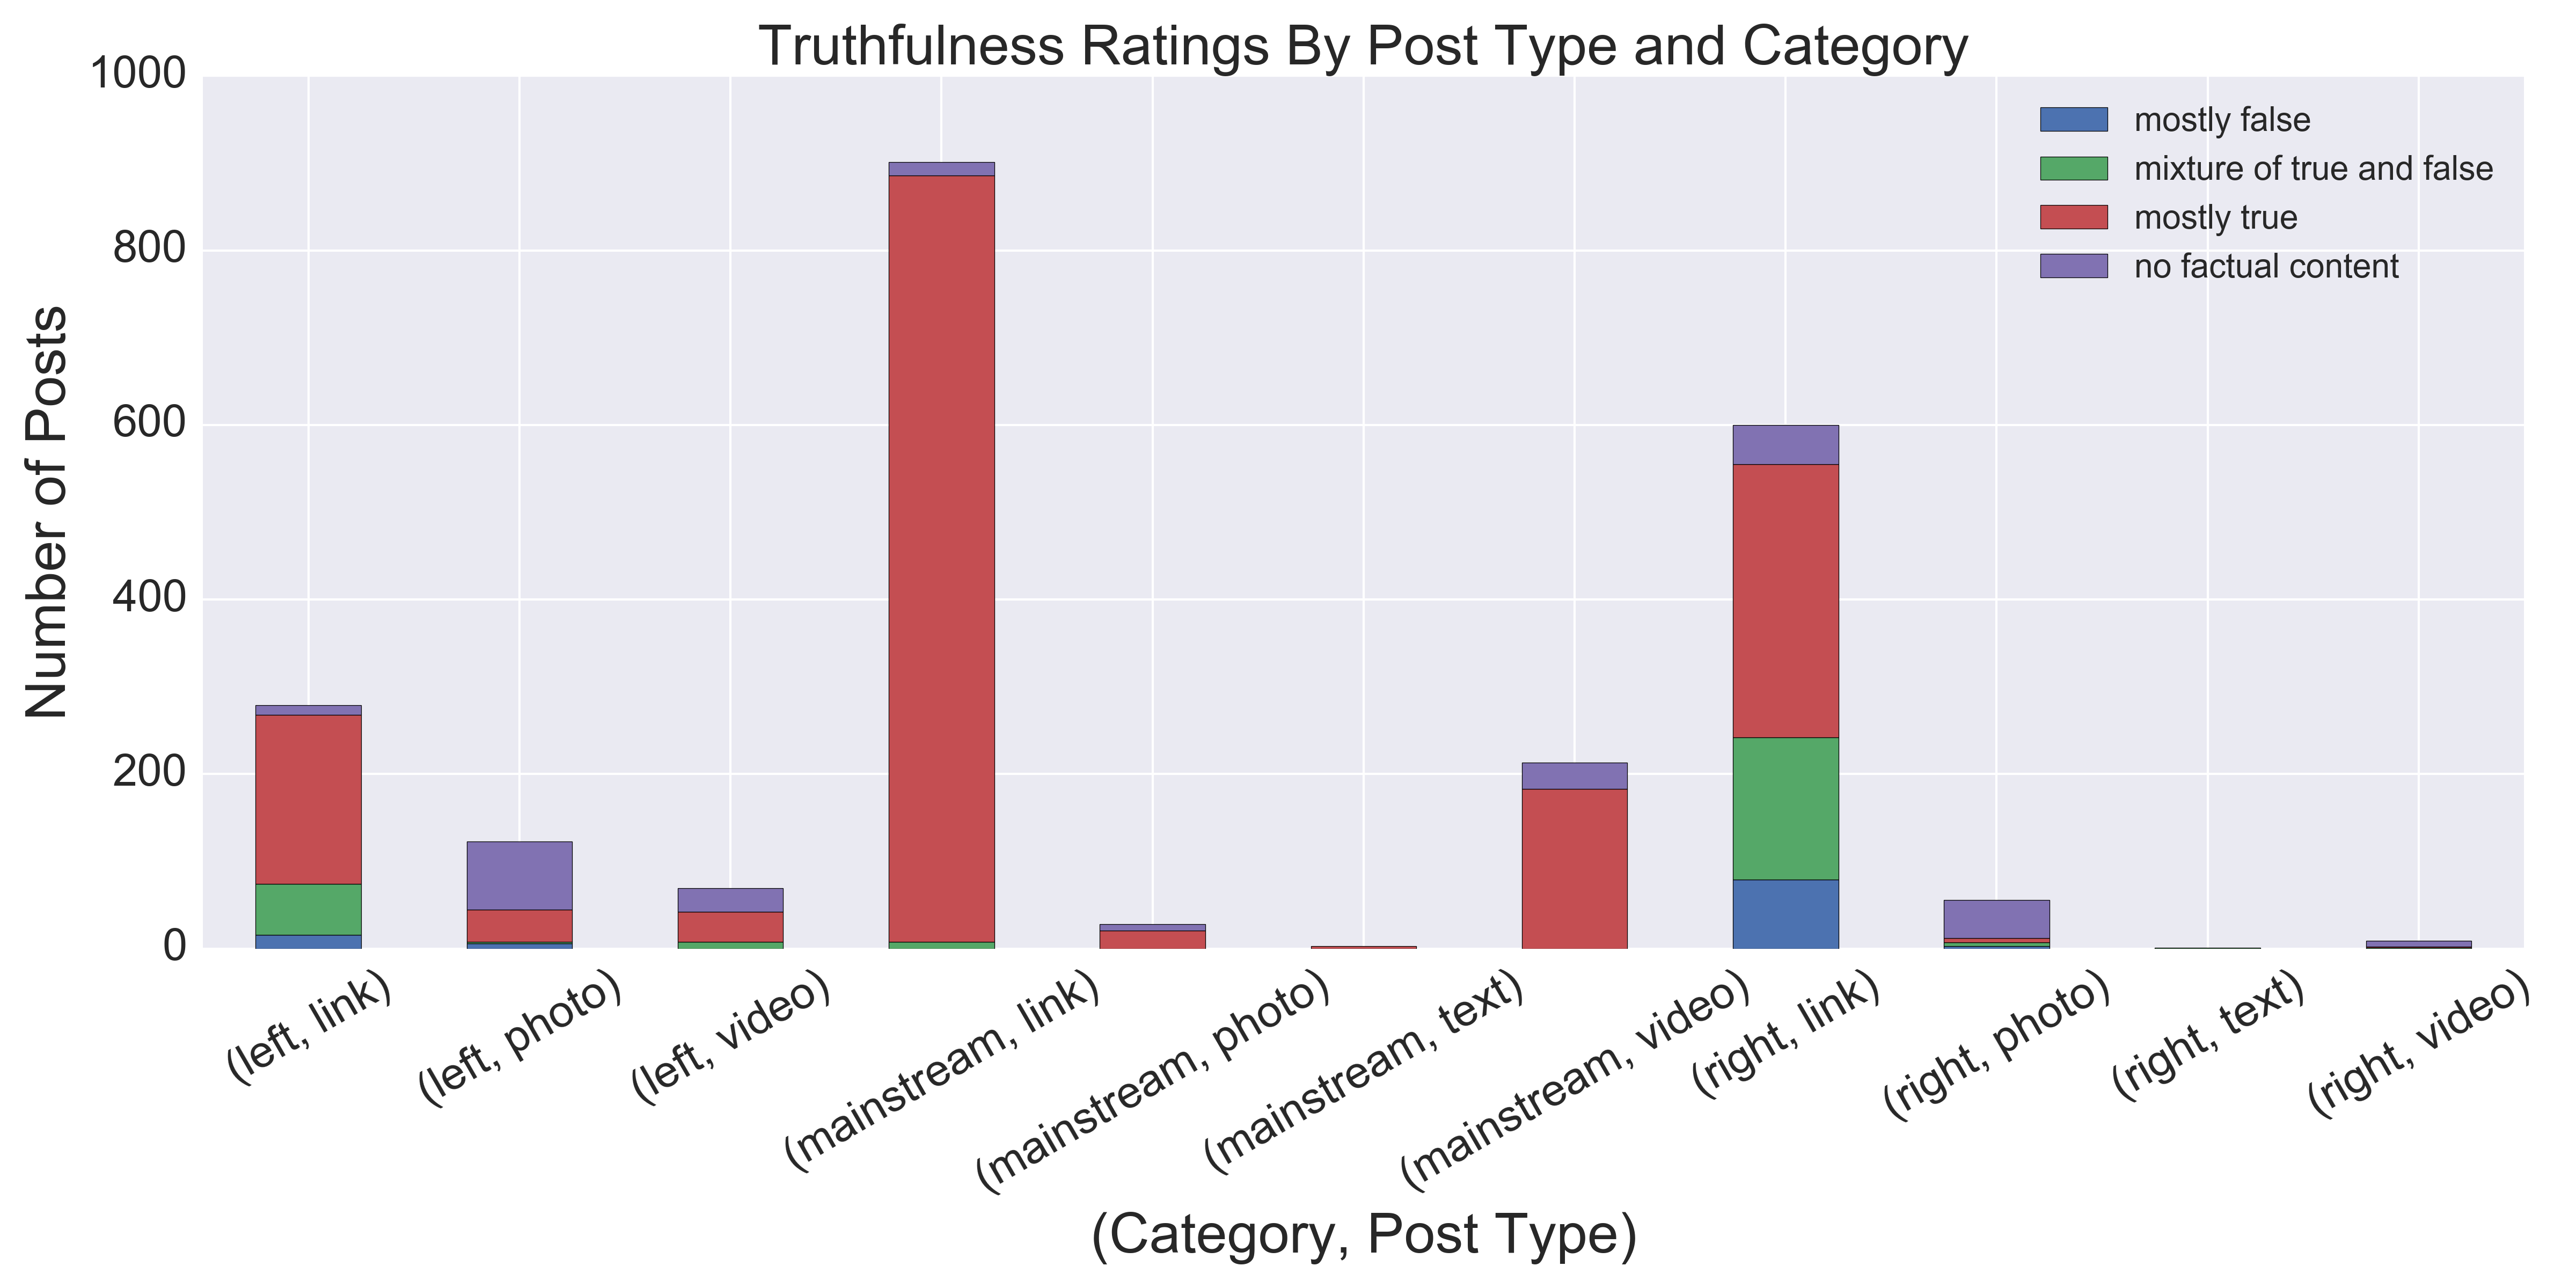
\includegraphics[width=\textwidth]{ratings_distribution_by_category_type.png}
\end{figure}

We first notice how much more common links are than any other post type. In order to get a better idea of the truthfulness breakdown by category, we visualize the percentage breakdown in each type instead of the relative counts. As the most popular post type, links initially appear more likely to be false or semi-false, but overall they have the highest truthfulness rating of any post type. Photos and videos are more likely to have no factual content than to be actually false, but text posts in this data set are universally mostly true if they come from a mainstream outlet, and a mixture of true and false from a right-wing outlet.
\begin{figure}[H] 
    \centering
    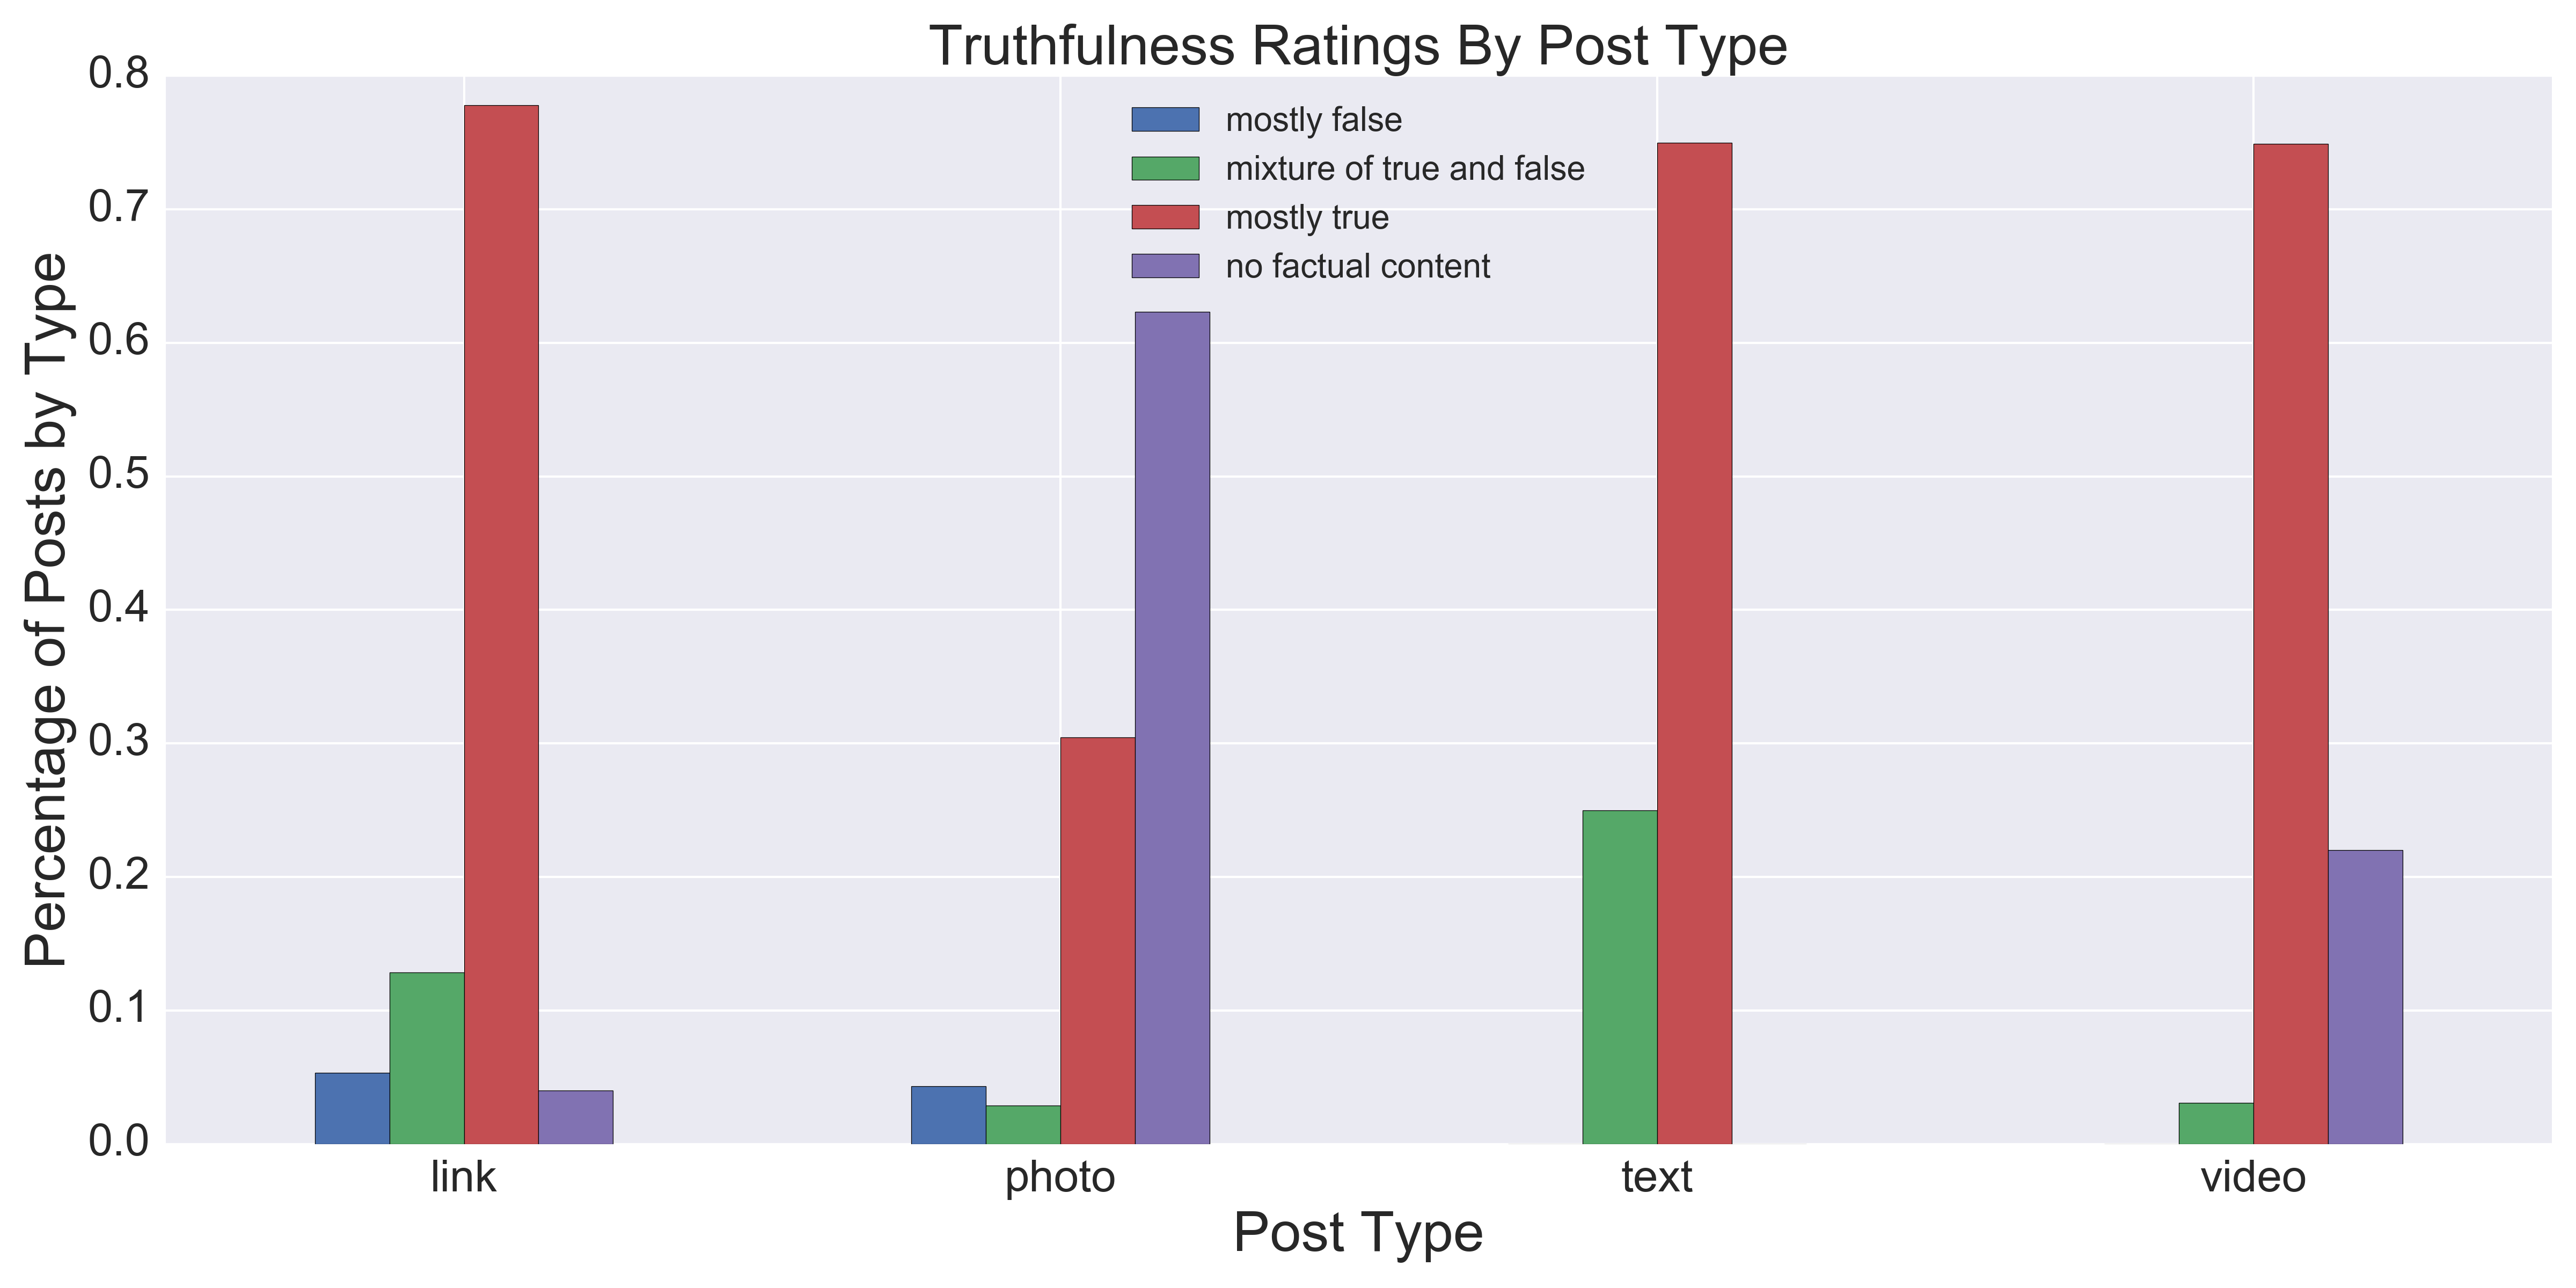
\includegraphics[width=\textwidth]{ratings_distribution_by_type.png}
\end{figure}

Finally, we investigate user engagement (shares, reactions, and comments).


\begin{figure}[H] 
    \centering
    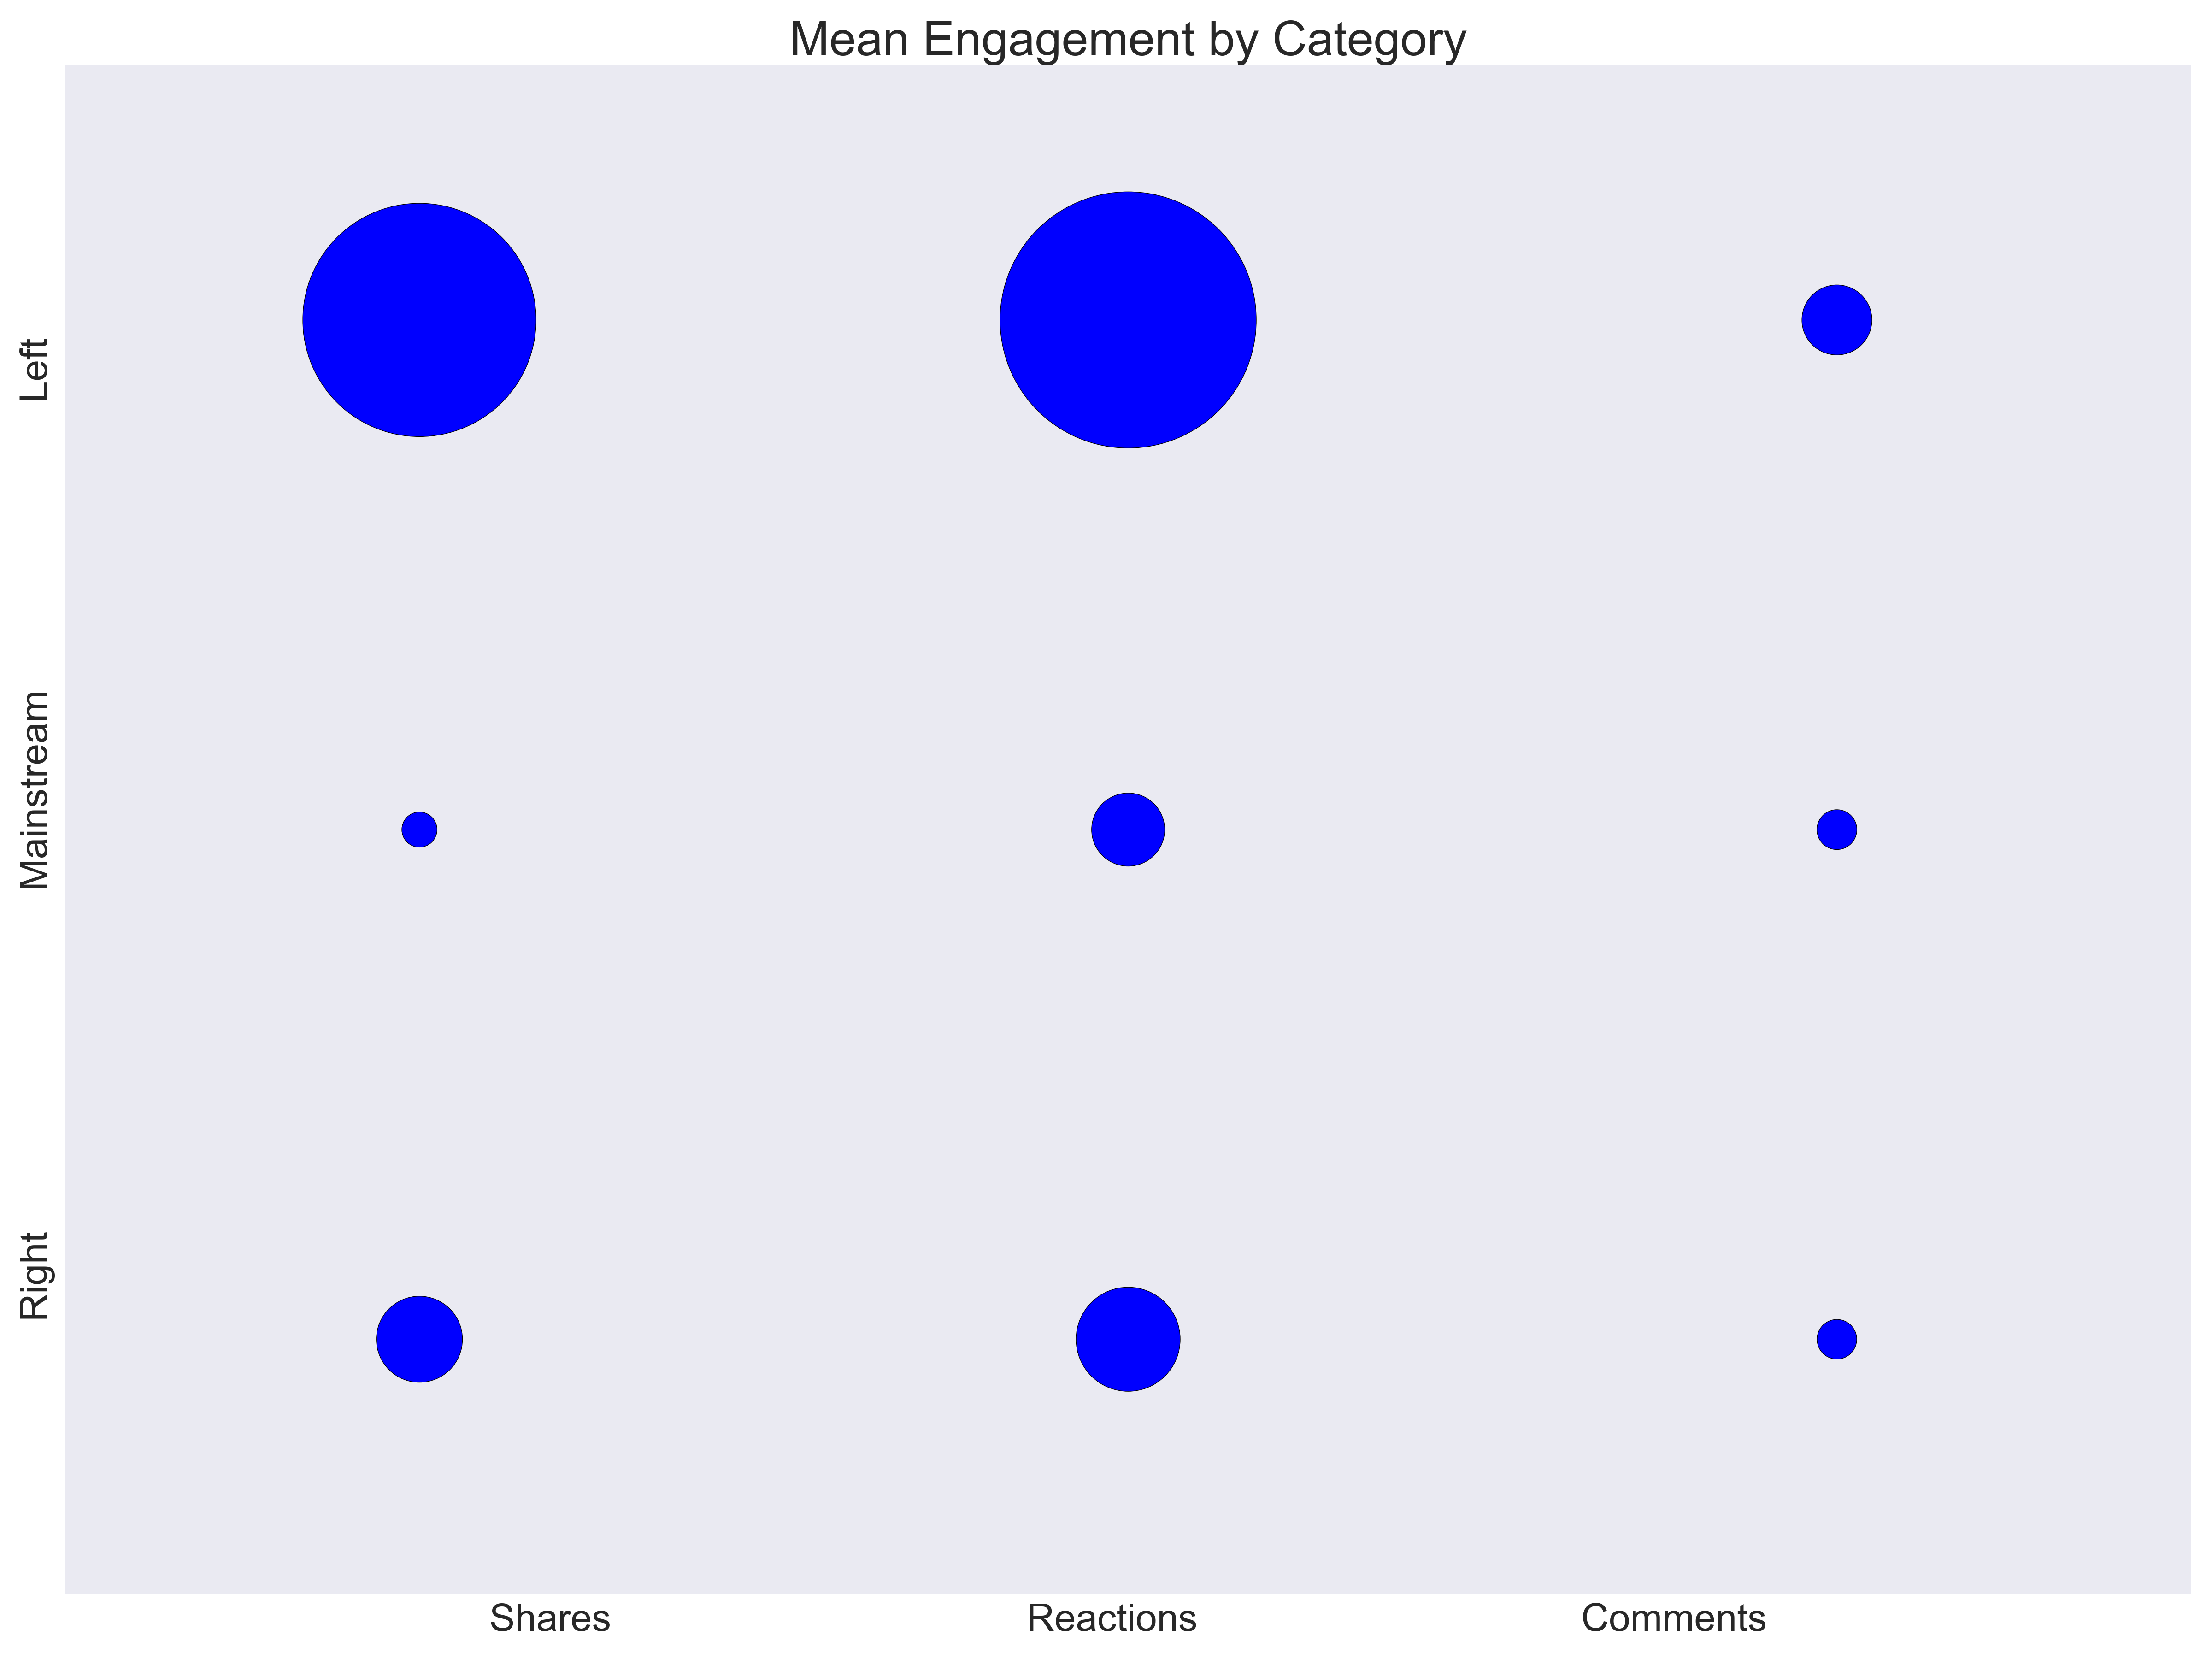
\includegraphics[width=0.75\textwidth]{engagement_by_category.png}
\end{figure}

\begin{figure}[H] 
    \centering
    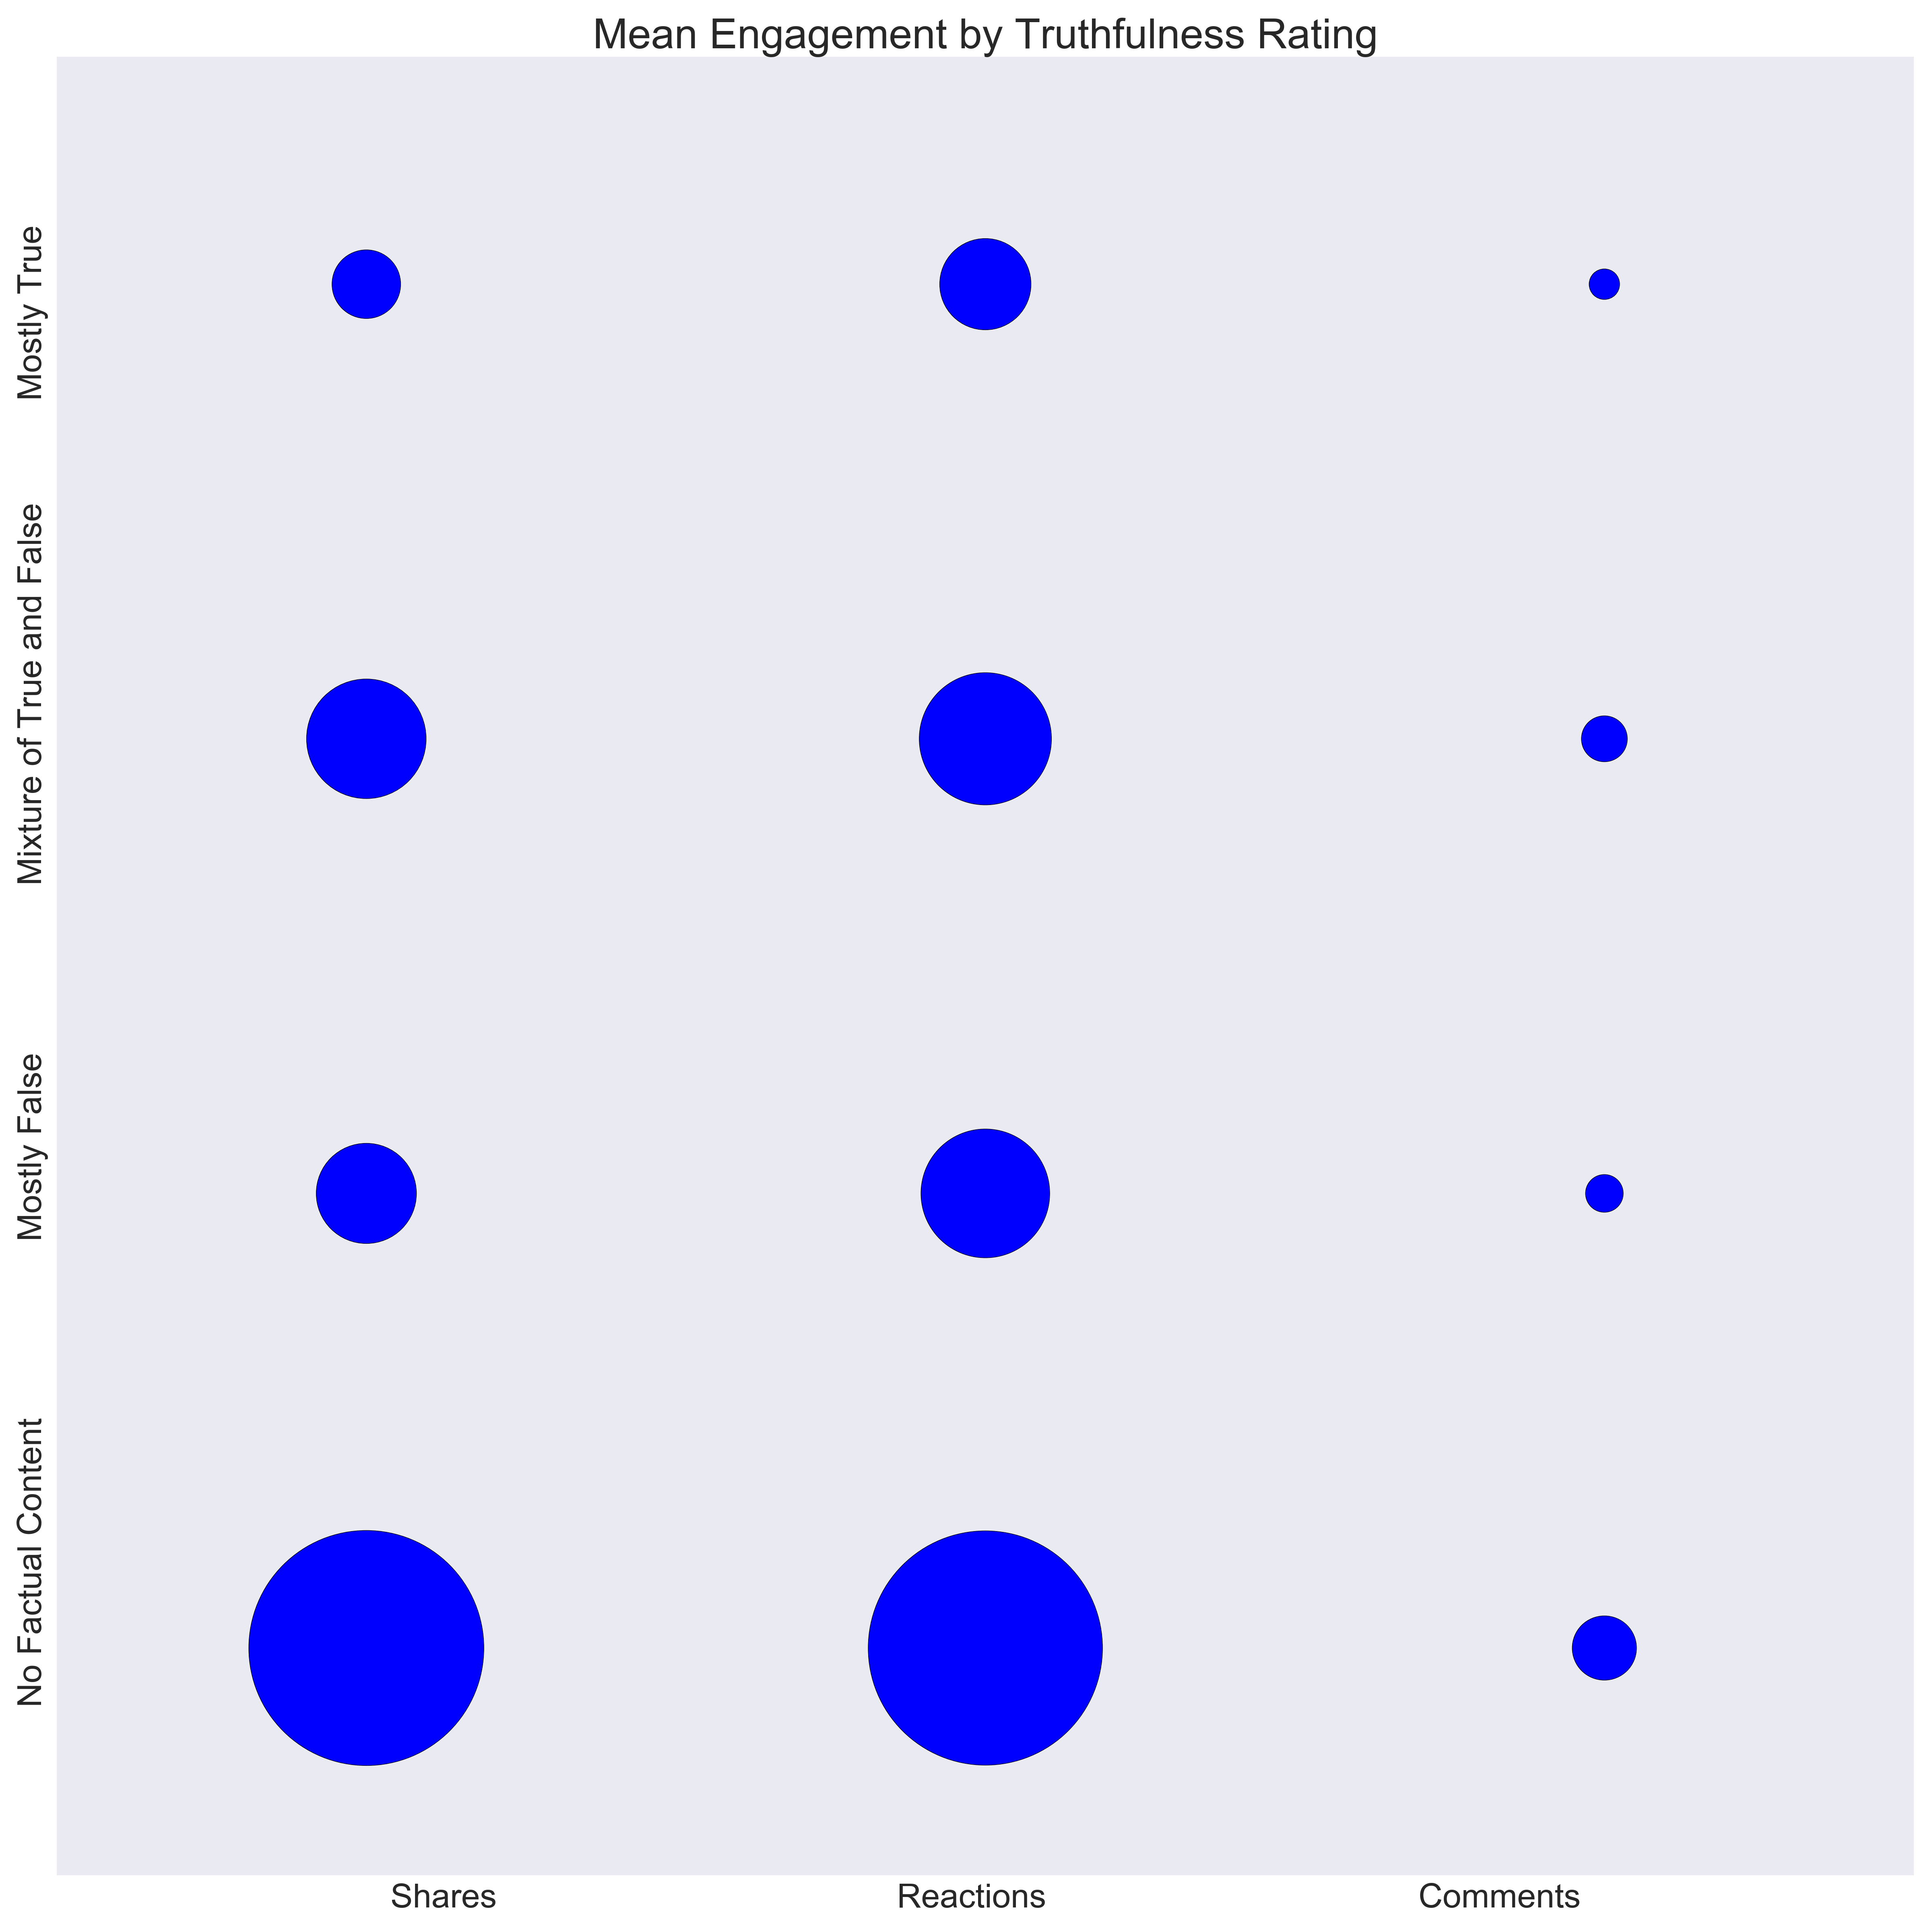
\includegraphics[width=0.75\textwidth]{engagement_by_truthfulness.png}
\end{figure}

We notice that engagement on posts (especially in terms of shares and reactions) is significantly higher for left-wing outlets, even after normalizing by the number of fans of the pages. While comments are lower across the board, there does not seem to be an overly significant difference between the relative numbers of shares, reactions, and comments between different truthfulness ratings.  Engagement is highest on posts with no factual content and posts which are a mixture of true and false. It looks as though both misleading posts and opinion/satirical posts are generally more popular than mostly true or mostly false posts.

\section*{Approach}

Since we did not observe a particularly strong relationship between mean engagement statistics of a post and truthfulness, we will ignore engagement statistics as we build our classifier. This gives our classifier the advantage of being able to predict the accuracy of a post as soon as it goes online, before it is able to mislead people. It also means all of our features (category, post type, date published, and post type) are categorical rather than continuous, which makes Naive Bayes a more natural fit for this problem. 

We will also build our classifier without using the date of publication. Since the goal is a classifier which makes predictions immediately upon publication, and we cannot know the effect of the date of publication on truthfulness until at least after that day is over, this feature is less helpful.


\subsection*{Naive Bayes}

We split the data into a training and test set by randomly choosing about 20\% of the rows in our dataframe as our test data, and leaving the rest as training data. 

We model the problem using a Naive Bayes classifier. Each post is represented by a bag of independent features which map to a truthfulness rating. Since the \texttt{Category} and \texttt{Page} features are not independent, the features we use for prediction in our classifier are \texttt{Post Type} and either \texttt{Category} or \texttt{Page}. We test our classifier for both cases, since a classifier based on the category of a news outlet can extend to a wider variety of new posts (that is, including news outlets we haven't seen yet) than predictions based on the pages themselves, but if this comes at a significant cost to accuracy it may not be worth it.

To train the classifier, we need to compute the probability that a post belongs to a certain class of truthfulness rating based on the post type and category or page. Using Bayes' theorem, we can compute this by multiplying the probabilities that a post has each feature, given the truthfulness rating. These probabilities can be found by counting the occurences of each feature, as in the following code.

\begin{lstlisting}
""" Return an array where A[i,j] is the probability of feature j given rating i."""
A = np.zeros((4, len(np.unique(data[column_name]))))

for j in np.unique(data[column_name]):
    # Count the number of times the rating occurs for each possible feature in the column
    A[:,j] = np.bincount(data[data[col_name]==j]['Rating'], minlength=4)

A = A / np.sum(A, axis=1)[:,np.newaxis] # Convert to probabilities
A[A == 0] = epsilon # Non-observed cases have probability epsilon
\end{lstlisting}

Now we can find the probability of each rating category for any given test point simply by multiplying over \texttt{A[i,j]}, where \texttt{i} is the rating index and \texttt{j} is the index of the feature of the test point. These probabilities can also be used for various alternative methods of flagging possible fake news.

\subsection*{Code Overview}

We read in the data as a Pandas Dataframe, and convert the categorical data into integers for easier processing. We define helper functions to calculate the RMSE, to calculate and display confusion matrices and overall error rates for the results, to split the data into test and training data, to calculate sensitivity and specificity, and to build the probability lookup tables  (as described in the above code).

We then build the probability tables at the heart of both the naive classifier and other flagging methods. This is fairly simple.
\begin{lstlisting}
# Build the probability lookup tables
page_probs, type_probs = build_probs(train_data, [`Page', `Post Type'])
cat_probs, type_probs = build_probs(train_data, [`Category', `Post Type'])

predict_page_probs = np.zeros((n,4))
predict_cat_probs = np.zeros((n,4))

# Estimate probability of each category for each test point
for i in xrange(n):
    test_pt = test_data.ix[all_inds[i]] # Get the test point
    
    for j in xrange(4): # For each truthfulness category
        
        page_ind = test_pt['Page'] # Get the feature indices
        cat_ind = test_pt['Category']
        type_ind = test_pt['Post Type']
        
        # P(C_i) = prod( P(A_j = v_j|C_i) )
        predict_page_probs[i,j] = page_probs[j,page_ind] * type_probs[j,type_ind]
        predict_cat_probs[i,j] = cat_probs[j,cat_ind] * type_probs[j,type_ind]
\end{lstlisting}

At this point, we simply use \texttt{np.argmax} to get the predictions from the Naive bayes classifier, and then use our helper functions to report and display the results. The various rules used for the flagging methods are similarly straightforward.

\section*{Results}
\subsection*{Initial Results}
A Naive Bayes classifier typically makes predictions by choosing the class with the highest probability. We report the results for both the predictions based on the category and post type and based on the page and post type in confusion matrices, and also find the overall accuracy rate.

\begin{figure}[H] 
    \centering
    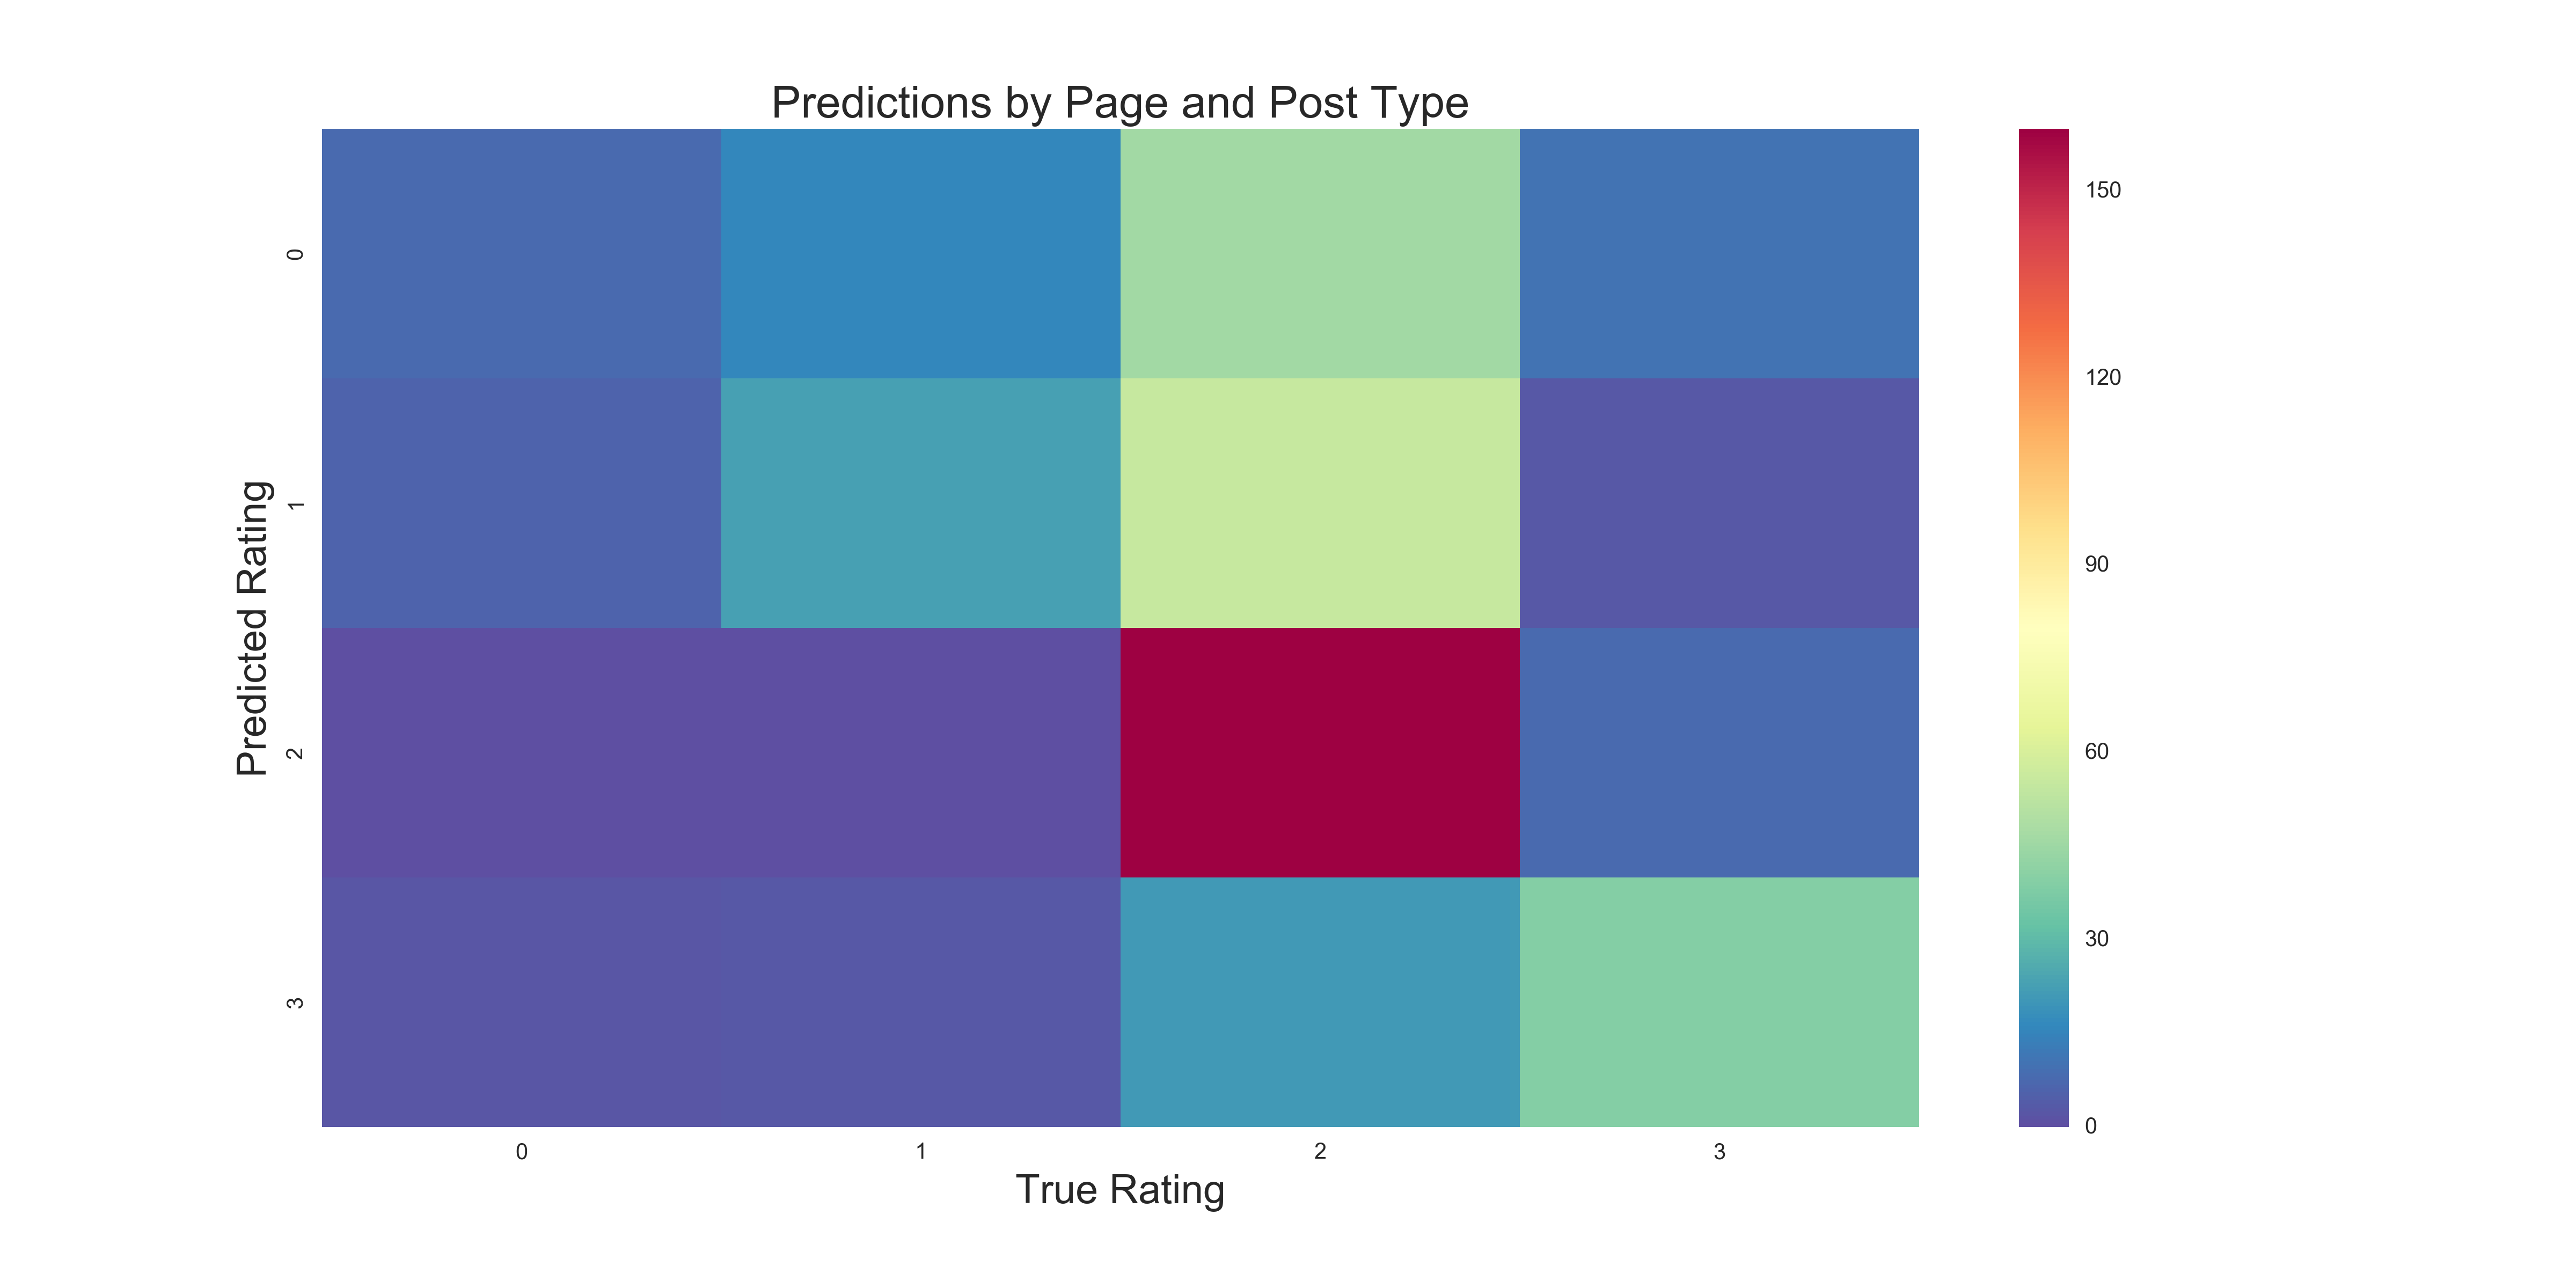
\includegraphics[width=0.93\textwidth]{page_predicts.png}
    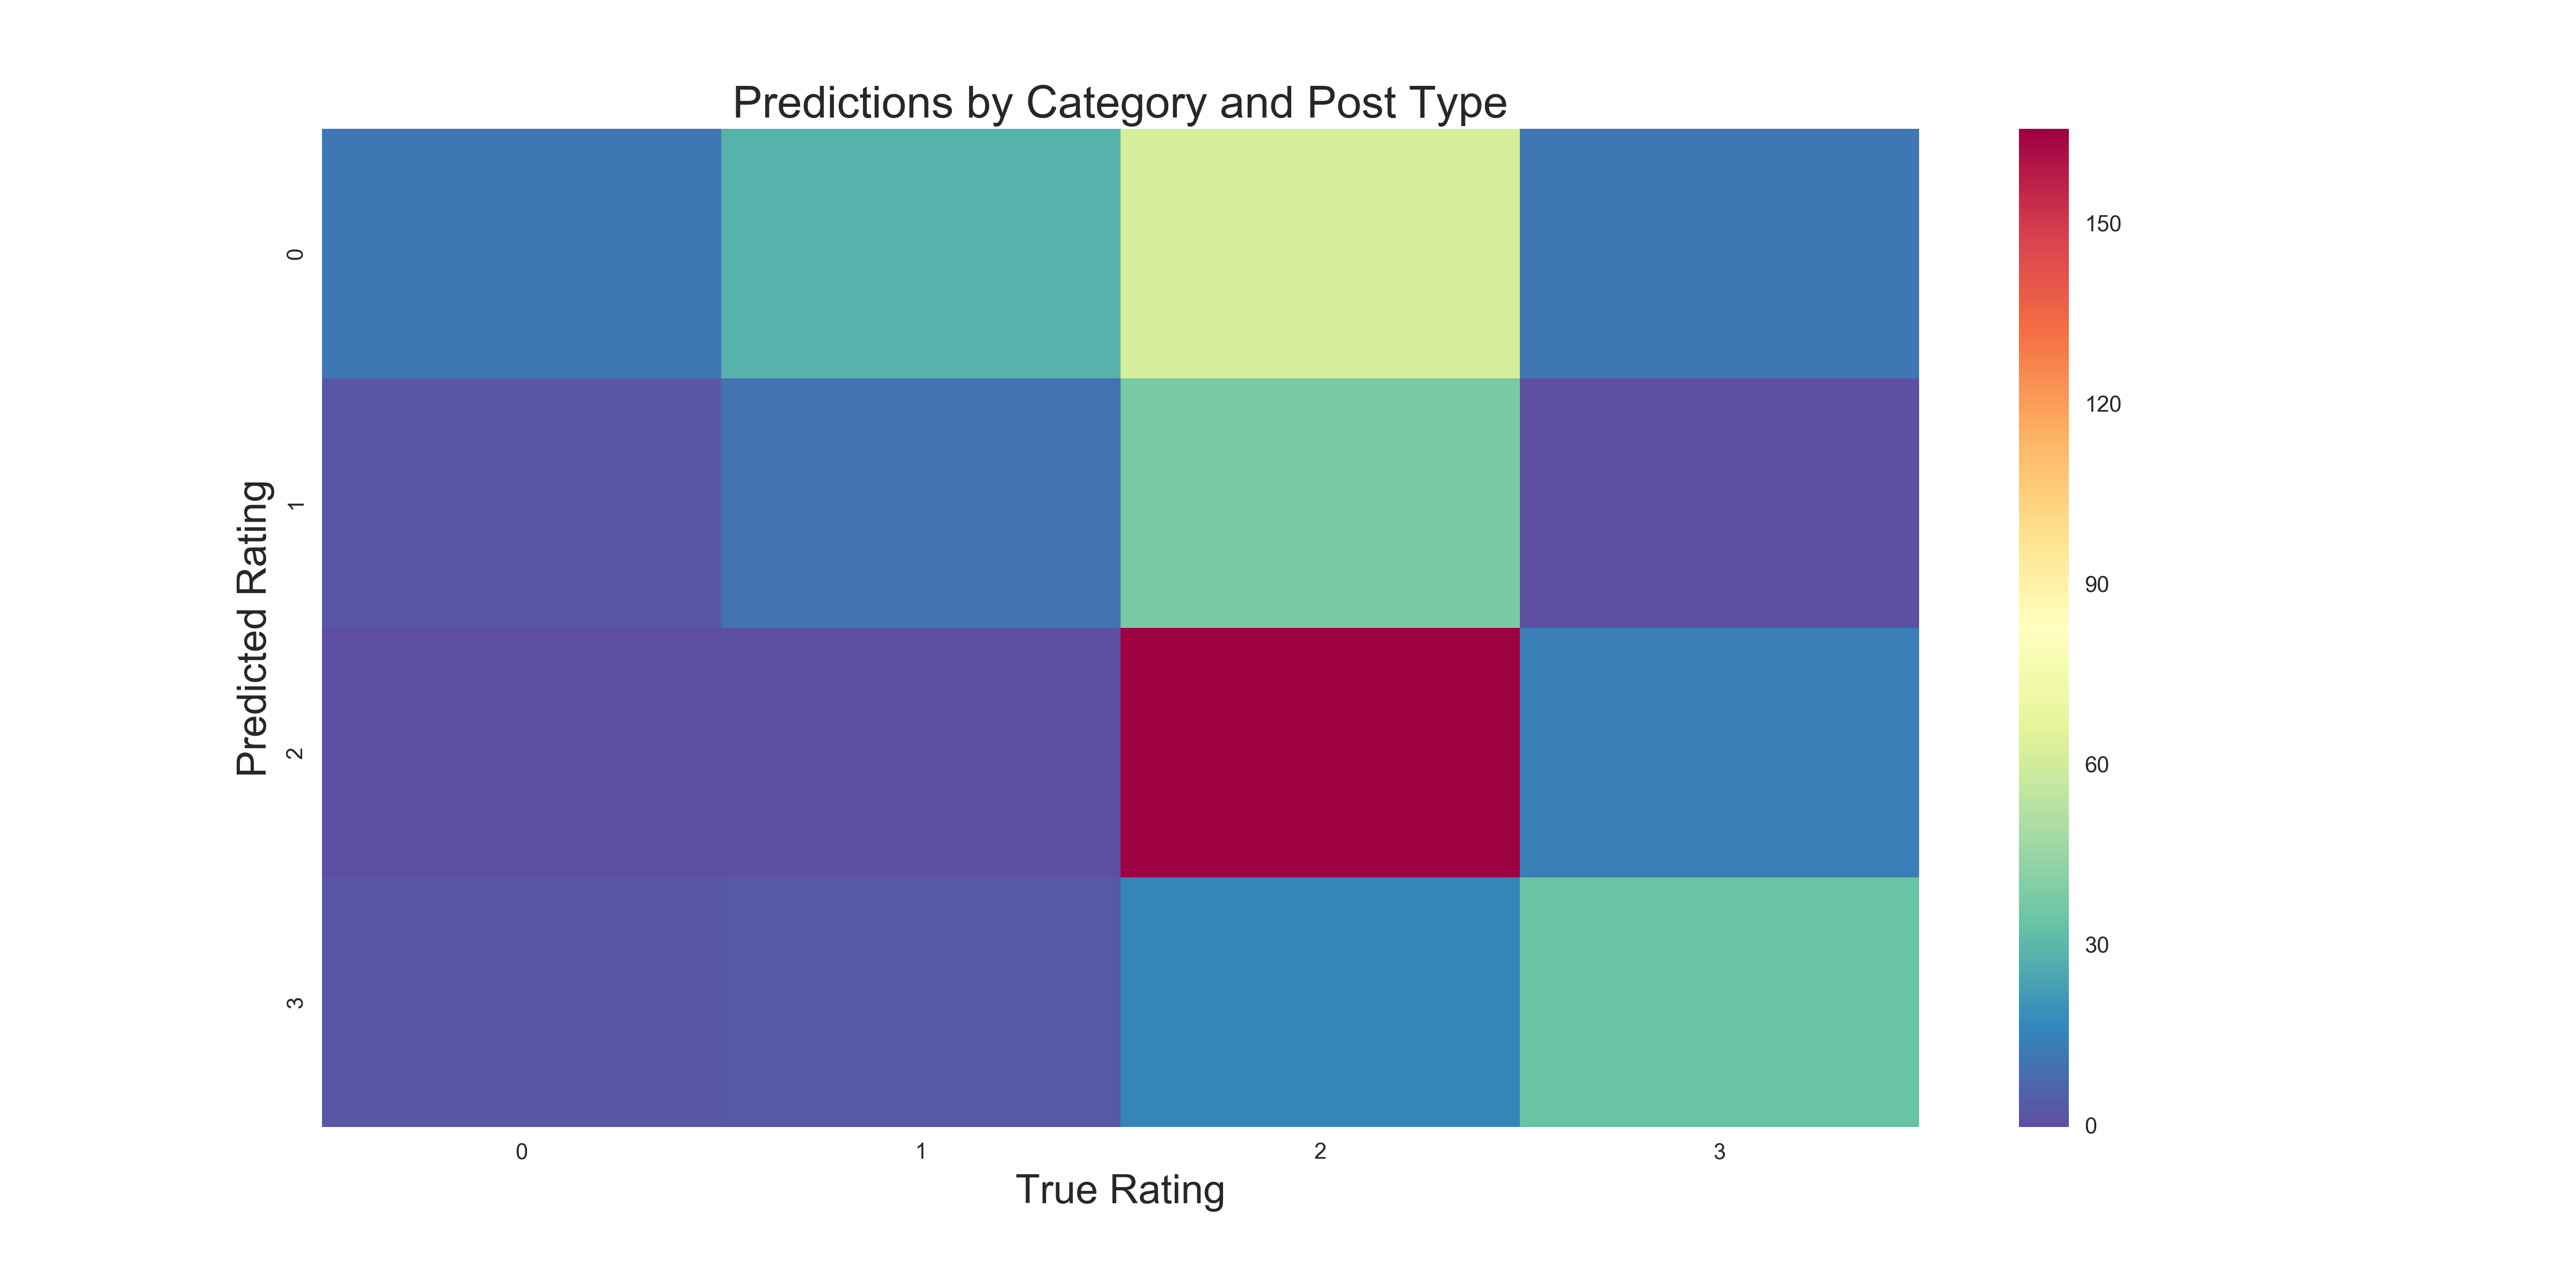
\includegraphics[width=0.93\textwidth]{cat_predicts.png}
\end{figure}

Since the dataset is small, variance in the error rate is fairly high and dependent on the initial test/train split of the data, but in general, the error rate hovers around 40\%, with the error rate for the predictions based on page and post type slightly better than the predictions based on category and post type. Varying the $\e$ used to compute the probabilities does not seem to help the error rate in any significant way. This is better than the 25\% we could expect from truly random guessing. However, since about 70\% of the posts are true regardless, we can get an error rate of under 30\% simply by marking every post as true. 

Attempting to measure the results using a modified RMSE that disproportionately penalizes marking true posts as false and vice versa also gives much better results for the ``assume everything is true" control classifier than our Naive Bayes. This tells us that we need to try something different.


\subsection*{Sensitivity and Specificity}

While it would be ideal to be able to perfectly predict the exact truthfulness rating of any given post, this does not appear to be feasible. Instead, since the overall goal is to detect false posts (which are relatively rare), we can treat this as a binary classification problem, similar to the breast cancer diagnosis problems used to illustrate Bayes' Theorem. We still use the probabilities obtained from the Naive Bayes model, but instead of choosing the maximum probability as the truthfulness rating, we attempt to diagnose posts which have a high probability of being false and our prediction is simply ``likely to be mostly false" and ``probably not mostly false".

In a real world situation, posts flagged as false could then be brought to the attention of human fact checkers, or readers could be given a warning that the post had a high probability of being false. We could also use the results to decide which posts to run through a more computationally expensive flagging method, since Naive Bayes is fairly cheap.

Performance is now measured by sensitivity and specificity. Sensitivity is the true positive rate, or the percentage of posts rated ``mostly false" which are flagged as false, while specificity is the true negative rate, or the posts that are not ``mostly false" which are not flagged as false. Since the main goal is narrow the set of possibly false posts without losing very many of them, we are mainly concerned with getting a high sensitivity rate.

The sensitivity and specificity results for various flagging techniques are summarized in the following table. We use the probability table based on category and post type.

Other probability thresholds besides those included were tested, but we only include those with meaningfully different sensitivities or specificities. We notice that several methods give the same results. Presumably this is a result of the small size of the dataset.

\begin{figure}[H]
\begin{center}
{\renewcommand{\arraystretch}{1.5}
\begin{tabular}{|| p{0.65\textwidth} | r | r ||}

\hline \hline
\textbf{Method} & \textbf{Sensitivity} & \textbf{Specificity} \\
\hline \hline

Report false always (positive control) & 100\% & 0\% \\ 
\hline
Report false never (negative control) & 0\% & 100\% \\
\hline
Report false if ``mostly false" has highest probability & 64.28\% & 74.87\% \\
\hline
Report false if ``mostly false" or ``mixture of true and false" has highest probability & 92.85\% & 61.6\% \\
\hline
Report false if ``mostly false" is highest or second highest probability & 100.00\% & 54.92\% \\
\hline
Report false if absolute probability of ``mostly false" is above 75\% & 0.00\% & 100.00\% \\
\hline 
Report false if absolute probability of ``mostly false" is above 50\% & 64.28\% & 74.87\% \\
\hline 
Report false if absolute probability of ``mostly false" is above 15\% & 92.85\% & 61.65\% \\
\hline 
Report false if absolute probability of ``mostly false" is above 5\% & 92.85\% & 59.32\% \\
\hline 
Report false if absolute probability of ``mostly false" is above 1\% & 100.00\% & 54.92\% \\
\hline 
Report false if normalized probability of ``mostly false" is above 50\% & 0.00\% & 100.00\% \\
\hline 
Report false if normalized probability of ``mostly false" is above 25\% & 92.85\% & 59.32\% \\
\hline 
Report false if normalized probability of ``mostly false" is above 1\% & 100.00\% & 54.92\% \\

\hline \hline
\end{tabular}
}
\end{center}
\end{figure}

\subsection*{Overfitting}

In order to check for overfitting, we run the prediction algorithm on a subset of the training of the same size as the test data and compare the error rate.

Again, we see a high amount of variance in the results after running the test for a few different training sets, but the error percentages are at most a few percent lower for the predictions on the training data, instead of dramatically different as they would be for an overfitted algorithm. We therefore can be reasonably sure we haven't overfitted the data.

We do not get different specificities and sensitivities when we test on training data, which is further evidence that we do not have a problem with overfitting.

\section*{Conclusion}

The first algorithm tried was fairly unsuccessful due to the limited predictive scope of the data used, so the binary classification methods were tried as a way to make more realistic use of the information available

Using these methods, we can get very good sensitivity ratings--between 90\% and 100\%--while keeping the specificity between 55\% and 62\%. Since there are many more non-false posts than false posts, this gives a very high false positive rate and does not seem encouraging. According to Bayes theorem, for these particular combinations, the false positive rate is high enough that a flagged post still only has about a 10\% chance of being false. Although this is low, it is still over twice the posterior probability of a given post being false.

Since this method is very cheap, it could be useful as an initial filter to decide which posts to track further using more computationally intensive methods. Such methods could include scanning headlines for certain keywords or scraping the contents of the link and scanning for certain keywords and using that method to flag which of the narrowed-down set of posts need to be checked manually or given a warning. It would also be fairly easy to modify the method to be easily updated as new data comes in and to check new posts against the training corpus one at a time as they are posted, making it potentially useful as a first filter against fake news.


\end{document}
